
\documentclass[11pt,a4paper]{article}

\usepackage[margin=1in]{geometry}
\usepackage[T1]{fontenc}
\usepackage[utf8]{inputenc}
\usepackage{lmodern}
\usepackage{microtype}
\usepackage{amsmath,amssymb}
\usepackage{booktabs}
\usepackage{enumitem}
\usepackage{hyperref}
\usepackage{xcolor}
\usepackage{listings}
\usepackage{fancyhdr}
\usepackage{titlesec}
\usepackage{graphicx}

\hypersetup{
    colorlinks=true,
    linkcolor=blue,
    urlcolor=blue,
    citecolor=blue
}

\definecolor{codegray}{gray}{0.95}

\lstset{
    basicstyle=\ttfamily\small,
    backgroundcolor=\color{codegray},
    frame=single,
    breaklines=true,
    columns=fullflexible,
    keepspaces=true,
    showstringspaces=false
}

\pagestyle{fancy}
\fancyhf{}
\lhead{FRC Research Notes}
\rhead{Week 2}
\cfoot{\thepage}

\titleformat{\section}{\large\bfseries}{\thesection.}{0.5em}{}
\titleformat{\subsection}{\normalsize\bfseries}{\thesubsection.}{0.5em}{}

\title{\textbf{FRC Research --- Week 2 Working Notes}\\
\large Baseline Reproduction, Audit, and Framework Design}
\author{Juan Pablo Solís Ruiz\\
Supervisor: Prof. Ren Haijun}
\date{September 2026}

\begin{document}

\maketitle
\tableofcontents
\newpage

\section{Purpose of These Notes}

These are living research notes for the second week of the FRC project. The immediate goal is to take over the inherited WarpX-based FRC workflow in a controlled way, reproduce its current baseline, and then progressively transform the workflow into a reproducible and extensible simulation framework.

The guiding principle for this stage is

\[
\boxed{\text{Reproduce} \;\rightarrow\; \text{Verify} \;\rightarrow\; \text{Refactor}}
\]

rather than modifying the inherited workflow before establishing a trusted reference result.

The long-term objective is not to maintain a single rigid input file or a collection of unrelated scripts. The target is a framework in which physical parameters, numerical parameters, HPC resources, diagnostics, provenance, and post-processing are clearly separated and can be changed systematically.

\section{Immediate Scientific and Engineering Objective}

The current short-term objective can be stated as:

\begin{quote}
\textit{Reproduce the inherited FRC baseline reliably and establish the first version of a reproducible case-management workflow.}
\end{quote}

This objective has two parallel components:

\begin{enumerate}[label=\arabic*.]
    \item \textbf{Scientific reproduction:} determine exactly what the inherited case does, reproduce it without changing the physics, and verify that the resulting diagnostics agree with the existing reference output.
    \item \textbf{Software and workflow engineering:} organize the case definition and execution workflow so that future formation, stability, merging, and compression studies do not depend on manually editing one large input file.
\end{enumerate}

The software work must not get ahead of the physics validation. A clean framework that does not reproduce the inherited result is not yet useful.

\section{Current SCNet Environment}

The inherited working area currently identified on SCNet is approximately:

\begin{lstlisting}
~/WQ/
|-- FRC/
|   |-- input_test
|   |-- run.sbatch
|   `-- results/
|       |-- i/
|       `-- j/
|
|-- WarpX/
|-- warpx-deps/
|-- tools/
|-- build.sbatch
`-- build.<jobid>.out
\end{lstlisting}

At present, the \texttt{WQ/FRC} directory appears to contain an FRC formation workflow rather than the Grad--Shafranov/tilt workflow that was previously studied locally.

The existing WarpX executable was built for:

\begin{itemize}
    \item 3D geometry,
    \item MPI,
    \item OpenMP,
    \item double precision,
    \item openPMD support,
    \item CPU execution.
\end{itemize}

The build configuration contains, in particular,

\begin{lstlisting}
-DWarpX_COMPUTE=OMP
-DWarpX_DIMS=3
-DWarpX_MPI=ON
\end{lstlisting}

Therefore, the inherited baseline is currently a CPU MPI+OpenMP workflow, not a CUDA/GPU workflow.

\subsection{Important preservation rule}

The inherited directories should be treated as a reference environment:

\begin{lstlisting}
~/WQ/FRC/
~/WQ/WarpX/
\end{lstlisting}

They should not be reset, updated, rebuilt, or cleaned until the baseline has been reproduced independently.

This is especially important because the current WarpX repository reports a \texttt{dirty} state. Therefore, the exact source tree used for the current executable may differ from a clean upstream WarpX checkout.

For the takeover phase, this environment should be treated as a \textbf{legacy baseline environment}.

\section{Observed Baseline Execution}

The two completed reference cases currently identified are labeled \texttt{i} and \texttt{j}.

Both used:

\begin{align*}
N_{\mathrm{MPI}} &= 4,\\
N_{\mathrm{OMP/rank}} &= 8,
\end{align*}

for a total of 32 CPU threads on one node.

The inherited Slurm configuration is approximately:

\begin{lstlisting}
#SBATCH -p kshcnormal
#SBATCH -N 1
#SBATCH --ntasks-per-node=4
#SBATCH -c 8
#SBATCH --exclusive
#SBATCH -t 8:00:00
\end{lstlisting}

The use of \texttt{--exclusive} means that the whole node is reserved. This is appropriate only after confirming the allocation/billing policy and after determining that the full node is actually useful.

The completed cases ran for roughly 2.6 hours.

The existing output already occupies tens of GB, so storage and diagnostic frequency must be treated as design parameters rather than afterthoughts.

\section{What Cases \texttt{i} and \texttt{j} Currently Mean}

A comparison of the two \texttt{warpx\_used\_inputs} files shows that the physical and numerical configurations are the same. The differences found so far are output paths such as

\begin{lstlisting}
results/i/<jobid>/...
results/j/<jobid>/...
\end{lstlisting}

Thus, at present, \texttt{i} and \texttt{j} act primarily as run labels rather than explicit physical case definitions.

This is an important workflow weakness. A future user should not have to ask:

\begin{quote}
``What did case \texttt{i} mean?''
\end{quote}

The case identity should instead be encoded in a structured configuration and recorded automatically with the output.

\section{Current Formation Input: Physical Interpretation}

The current \texttt{input\_test} defines an initially negative axial bias field

\[
B_0 = -0.08\;\mathrm{T},
\]

and a driven field with target scale

\[
B_{\max}=0.13\;\mathrm{T}.
\]

The drive is ramped over

\[
t_{\mathrm{peak}} = 4~\mu\mathrm{s}.
\]

The ion species is labeled \texttt{protons}, but the assigned mass is approximately twice the proton mass, corresponding to deuterium ions.

Other representative physical parameters include:

\[
n_0 = 5\times 10^{19}\;\mathrm{m}^{-3},
\]

\[
T_e = T_i = 5\;\mathrm{eV}.
\]

The present grid and timestep are approximately

\[
N_x\times N_y\times N_z = 64\times64\times192,
\]

with additional axial PML cells, and

\[
\Delta t = 1~\mathrm{ns}.
\]

The current input uses

\[
N_t=2000,
\]

so the simulated physical duration is only

\[
t_{\mathrm{end}} = N_t\Delta t = 2~\mu\mathrm{s}.
\]

Therefore, the present test case stops before the nominal \(4~\mu\mathrm{s}\) field ramp is complete. This is evidence that the current file is likely a development/test configuration rather than a complete formation study.

\section{Why the Existing Input Needs Auditing}

The current input is valuable because it represents the working inherited model, but it mixes several kinds of information:

\begin{itemize}
    \item physical parameters,
    \item geometry,
    \item numerical resolution,
    \item algorithm choices,
    \item boundary conditions,
    \item diagnostic settings,
    \item implementation comments,
    \item experimental/development remnants.
\end{itemize}

Some comments also appear to be older than the values currently used. For example, a parameter may contain one numerical value while the adjacent comment describes a different previous value.

For this reason:

\begin{quote}
\textbf{The executed input and \texttt{warpx\_used\_inputs} are authoritative; comments are explanatory but must be verified.}
\end{quote}

\section{Framework Design Goal}

The future framework should separate at least four parameter layers.

\subsection{Physics}

Examples:

\begin{itemize}
    \item density,
    \item electron temperature,
    \item ion temperature,
    \item bias magnetic field,
    \item driven magnetic field,
    \item field rise time,
    \item resistivity/hyper-resistivity model,
    \item perturbation amplitudes when relevant.
\end{itemize}

\subsection{Geometry}

Examples:

\begin{itemize}
    \item chamber radius,
    \item axial length,
    \item mirror geometry,
    \item physical simulation domain,
    \item embedded boundaries,
    \item PML placement.
\end{itemize}

\subsection{Numerics}

Examples:

\begin{itemize}
    \item \(N_x,N_y,N_z\),
    \item timestep,
    \item particles per cell,
    \item particle shape,
    \item filtering,
    \item load balancing,
    \item diagnostic cadence,
    \item checkpoint cadence,
    \item solver-specific parameters.
\end{itemize}

\subsection{Runtime / HPC}

Examples:

\begin{itemize}
    \item cluster/partition,
    \item number of nodes,
    \item MPI ranks,
    \item OpenMP threads,
    \item walltime,
    \item executable path,
    \item module environment.
\end{itemize}

These groups should not be hidden inside one monolithic file when systematic parameter studies begin.

\section{Single Source of Truth for a Case}

The desired design is that one structured configuration defines a physical/numerical case.

A possible future representation could be:

\begin{lstlisting}
[case]
name = "formation_baseline"

[physics]
n0 = 5.0e19
Te_eV = 5.0
Ti_eV = 5.0
B0_T = -0.08
Bmax_T = 0.13
t_peak_s = 4.0e-6

[geometry]
rm_m = 0.336
Lz_m = 2.56

[numerics]
Nx = 64
Ny = 64
Nz = 192
particles_per_cell = 200
dt_s = 1.0e-9
steps = 2000

[hpc]
mpi_ranks = 4
omp_threads = 8
\end{lstlisting}

The exact format is not yet fixed. TOML, YAML, or another simple structured format could work. The important point is the architecture: a case definition should be machine-readable, version-controlled, and independent from the generated WarpX input.

\section{Input Generation Philosophy}

The future framework should \textbf{not hide WarpX}.

Instead, the pipeline should be:

\begin{lstlisting}
case configuration
        |
        v
validation / derived quantities
        |
        v
generated WarpX input
        |
        v
Slurm submission
        |
        v
WarpX
        |
        v
diagnostics
\end{lstlisting}

The generated WarpX input should remain a normal, readable text file. This gives two advantages:

\begin{enumerate}[label=\arabic*.]
    \item the simulation can always be audited directly;
    \item debugging does not depend on understanding an opaque wrapper.
\end{enumerate}

Python should help generate and validate inputs, not make the underlying WarpX model inaccessible.

\section{Validation Layer}

Before a case is submitted, the framework should eventually perform automated checks.

Simple examples:

\begin{lstlisting}[language=Python]
assert Nx > 0
assert Ny > 0
assert Nz > 0
assert dt > 0.0
assert particles_per_cell > 0
assert max_step > 0
\end{lstlisting}

More useful FRC/WarpX-specific checks could include:

\begin{itemize}
    \item grid divisibility and blocking constraints,
    \item PML thickness relative to grid spacing,
    \item diagnostic intervals relative to total steps,
    \item consistency between physical domain and particle initialization domain,
    \item total simulated physical time,
    \item estimated number of macroparticles,
    \item estimated output size,
    \item estimated computational cost,
    \item warnings for suspiciously expensive settings.
\end{itemize}

This validation layer is important for both numerical reliability and HPC cost control.

\section{Run Provenance}

Every production run should be self-describing.

A future run manifest could contain information such as:

\begin{lstlisting}
case_name: formation_baseline
case_id: formation_baseline-a81f3c
created: 2026-09-17T...
git_commit: ...
warpx_version: 26.04-8-gb0e686a
input_sha256: ...
slurm_job_id: ...
partition: kshcnormal
nodes: 1
mpi_ranks: 4
omp_threads: 8
\end{lstlisting}

A run directory could then look like:

\begin{lstlisting}
results/
`-- formation_baseline-a81f3c/
    `-- <slurm-job-id>/
        |-- manifest.json
        |-- input
        |-- warpx_used_inputs
        |-- slurm.out
        |-- diag...
        `-- analysis/
\end{lstlisting}

This avoids ambiguous case names and makes comparison between simulations much safer.

\section{Possible Repository Evolution}

The existing research repository can evolve toward something like:

\begin{lstlisting}
frc-research/
|-- configs/
|   |-- formation/
|   |   |-- baseline.toml
|   |   `-- smoke.toml
|   `-- tilt/
|       `-- baseline.toml
|
|-- src/
|   `-- frc/
|       |-- config.py
|       |-- validation.py
|       |-- input_generator.py
|       |-- run_manifest.py
|       `-- analysis/
|
|-- templates/
|   |-- warpx_formation.in
|   |-- warpx_gs.in
|   `-- scnet_cpu.sbatch
|
|-- scripts/
|   |-- generate_case.py
|   |-- submit_case.py
|   |-- inspect_case.py
|   `-- analyze_case.py
|
|-- tests/
|-- docs/
`-- cases/
\end{lstlisting}

This is a target architecture, not an instruction to create every file immediately.

\section{Possible User Workflow}

Once the framework matures, the intended workflow could become approximately:

\begin{lstlisting}
frc generate configs/formation/baseline.toml
frc submit formation_baseline-a81f3c
frc status
frc analyze formation_baseline-a81f3c
\end{lstlisting}

The exact command-line interface is not important yet. The important idea is that case generation, submission, inspection, and analysis become standardized operations.

\section{Development Strategy}

The implementation should proceed in stages.

\subsection{Phase A --- Audit the inherited baseline}

Determine:

\begin{itemize}
    \item exactly what input was executed,
    \item what \texttt{i} and \texttt{j} represent,
    \item the WarpX/AMReX/PICSAR versions,
    \item physical runtime,
    \item computational runtime,
    \item CPU layout,
    \item disk usage,
    \item diagnostic cadence,
    \item output contents,
    \item whether existing outputs are scientifically usable.
\end{itemize}

No physics changes should be introduced in this phase.

\subsection{Phase B --- Create an independent smoke-test case}

Create a new user-controlled working area without changing the inherited files.

The smoke test should:

\begin{itemize}
    \item use the inherited executable,
    \item preserve the relevant model,
    \item run only a small number of steps,
    \item generate minimal diagnostics,
    \item verify that the execution path works,
    \item verify output directory handling,
    \item verify that the run can be reproduced.
\end{itemize}

\subsection{Phase C --- Reproduce the full baseline}

After the smoke test is trusted:

\begin{itemize}
    \item reproduce the inherited baseline,
    \item compare key diagnostics,
    \item compare runtime and resource use,
    \item document discrepancies,
    \item establish the reference result for subsequent development.
\end{itemize}

\subsection{Phase D --- Framework v0.1}

Only after baseline reproduction:

\begin{itemize}
    \item introduce structured case configuration,
    \item generate WarpX input from a template,
    \item generate run manifests,
    \item automate output organization,
    \item create minimal validation checks,
    \item preserve exact baseline reproducibility.
\end{itemize}

\subsection{Phase E --- Optimization and scientific parameter studies}

Only after correctness is established:

\begin{itemize}
    \item benchmark MPI/OpenMP layouts,
    \item investigate diagnostic cost,
    \item reduce unnecessary output,
    \item test alternative resolutions,
    \item evaluate CPU versus possible GPU builds if justified,
    \item begin controlled physical parameter scans.
\end{itemize}

Optimization should never change the reference physics silently.

\section{Week 2 Deliverable}

A realistic Week 2 deliverable is:

\begin{quote}
\textbf{Reproduce the inherited FRC formation baseline and establish the first version of a reproducible case-management workflow.}
\end{quote}

A successful week does not require a complete production framework.

A strong Week 2 result would include:

\begin{enumerate}[label=\arabic*.]
    \item a documented audit of the inherited case;
    \item a clear map of the SCNet execution environment;
    \item an independent smoke test;
    \item a first reproducible baseline run or a clearly documented reason why reproduction is blocked;
    \item a proposed architecture for the future framework;
    \item provenance recorded for every new run.
\end{enumerate}

\section{Current Open Questions}

The following questions remain active:

\begin{enumerate}[label=\arabic*.]
    \item What were the original scientific purposes of cases \texttt{i} and \texttt{j}?
    \item Are the existing \texttt{i}/\texttt{j} outputs intended as identical reproducibility tests, or was some distinction made outside the recorded WarpX input?
    \item What diagnostics are present inside the existing \texttt{diag} output?
    \item Is the current \(2000\)-step input intentionally truncated before the full field ramp?
    \item What is the intended complete formation runtime?
    \item Which quantities were used previously to judge successful FRC formation?
    \item What are the SCNet allocation/billing constraints for \texttt{kshcnormal}?
    \item Is \texttt{--exclusive} required or simply inherited from previous testing?
    \item Should the final framework support both formation and Grad--Shafranov/tilt workflows under the same case-management layer?
    \item Which parts of the inherited WarpX tree are intentionally modified relative to upstream?
\end{enumerate}

\section{Audit Checklist}

\begin{itemize}[label=$\square$]
    \item Record exact WarpX commit/version.
    \item Record AMReX and PICSAR versions.
    \item Preserve inherited executable checksum.
    \item Preserve inherited \texttt{input\_test}.
    \item Preserve inherited \texttt{run.sbatch}.
    \item Inspect complete \texttt{warpx\_used\_inputs}.
    \item Compare \texttt{i} and \texttt{j}.
    \item Inspect diagnostic directory structure.
    \item Measure run duration and output size.
    \item Identify dominant runtime costs if profiler data are available.
    \item Confirm checkpoint structure.
    \item Confirm whether the existing output can be post-processed.
    \item Establish a minimal scientific comparison quantity.
    \item Create independent JPSR working directory.
    \item Define a smoke-test configuration.
    \item Run smoke test.
    \item Reproduce baseline.
    \item Begin framework v0.1 only after reproduction.
\end{itemize}

\section{Research Log}

\subsection*{2026-09-17}

\begin{itemize}
    \item Confirmed functional SSH access to SCNet.
    \item Identified inherited FRC and WarpX directories under \texttt{\textasciitilde/WQ}.
    \item Confirmed CPU MPI+OpenMP WarpX build.
    \item Identified two previous runs, \texttt{i} and \texttt{j}.
    \item Confirmed both use 4 MPI ranks and 8 OpenMP threads per rank.
    \item Observed that their recorded WarpX inputs differ only in output paths.
    \item Confirmed the current WarpX tree is not clean and should therefore be preserved as a legacy reference.
    \item Defined the development strategy: reproduce, verify, then refactor.
    \item Defined the preliminary architecture for a future FRC simulation framework.
\end{itemize}

\subsection*{Next entry}

Continue with the detailed baseline audit:
\begin{itemize}
    \item inspect complete run outputs and diagnostics;
    \item identify the scientific meaning of the existing result;
    \item establish the minimum quantities needed for baseline comparison;
    \item prepare an independent smoke-test case.
\end{itemize}

\section{Baseline Audit Results}

The inherited FRC workflow on SCNet has now been inspected sufficiently to establish a first reproducibility strategy. The main objective of this audit was to determine what was actually executed, how the existing runs differ, how the WarpX executable was built, and which parts of the workflow should be preserved as a reference before beginning independent development.

\subsection{Inherited WarpX Environment}

The current WarpX executable corresponds to

\begin{lstlisting}
WarpX 26.04-8-gb0e686a
commit: b0e686a
\end{lstlisting}

and was built for a three-dimensional CPU configuration using MPI and OpenMP:

\begin{lstlisting}
-DWarpX_COMPUTE=OMP
-DWarpX_DIMS=3
-DWarpX_MPI=ON
\end{lstlisting}

The executable used by the FRC jobs is a symbolic link:

\begin{lstlisting}
warpx.3d
    -> warpx.3d.MPI.OMP.DP.PDP.OPMD.EB.QED
\end{lstlisting}

Thus, the inherited workflow is a CPU-based hybrid MPI/OpenMP configuration rather than a CUDA/GPU workflow.

Initially, the WarpX repository appeared to contain a very large number of modified files and WarpX reported itself as \texttt{dirty}. However, a global comparison that ignores end-of-line whitespace returned

\begin{lstlisting}
git diff --ignore-space-at-eol --quiet
echo $?
0
\end{lstlisting}

indicating that no content differences were detected once end-of-line changes were ignored.

The current interpretation is therefore:

\begin{quote}
The inherited WarpX source tree is consistent with commit \texttt{b0e686a}; the apparent dirty state is caused by line-ending differences rather than identified changes to the physical solver source code.
\end{quote}

This is important because it means the present executable can be treated as a relatively well-defined legacy reference without assuming the existence of a heavily customized WarpX fork.

\subsection{Reference Runs \texttt{i} and \texttt{j}}

Two completed FRC runs were identified:

\begin{lstlisting}
results/i/111646811
results/j/111646815
\end{lstlisting}

Both runs used the same computational configuration:

\begin{align*}
N_{\mathrm{MPI}} &= 4,\\
N_{\mathrm{OMP/rank}} &= 8,
\end{align*}

for a total of 32 CPU cores on a single node.

Both runs also used the same physical and numerical WarpX input. A comparison of their respective \texttt{warpx\_used\_inputs} files showed differences only in output paths and run-specific metadata.

Therefore, \texttt{i} and \texttt{j} are not two different physical parameter cases.

Their computational runtime was approximately

\[
2.6~\mathrm{h}
\]

for 2000 timesteps.

\subsection{Evidence for Node-Reproducibility Testing}

A separate tool was found in

\begin{lstlisting}
~/WQ/tools/
\end{lstlisting}

named

\begin{lstlisting}
node_repro_test.py
\end{lstlisting}

whose explicit purpose is to compare deterministic floating-point calculations across different SCNet compute nodes.

The test was executed on six Hygon C86 7185 nodes. All six produced the same numerical SHA-256 fingerprint:

\begin{lstlisting}
dec3903b35128c7870408b0453b51ce24d474d014d1b56a0a70961dc58b3f90b
\end{lstlisting}

and the test concluded that the deterministic numerical fingerprints were identical.

This provides evidence that cross-node floating-point behavior was being investigated in the inherited work. Since the FRC cases \texttt{i} and \texttt{j} were also launched with identical inputs on different nodes, it is plausible that they were part of a related reproducibility study.

However, this interpretation is not yet treated as a documented fact because no explicit note was found stating that \texttt{i} and \texttt{j} were themselves the WarpX node-reproducibility experiment.

\subsection{Diagnostic Structure and Storage Cost}

Each reference run contains 21 field diagnostics:

\begin{lstlisting}
diag000000
diag000100
diag000200
...
diag001900
diag002000
\end{lstlisting}

corresponding to one output every 100 timesteps.

Each plotfile is approximately

\[
72~\mathrm{MB}.
\]

The recorded variables are:

\begin{align*}
&B_x,\;B_y,\;B_z,\\
&E_x,\;E_y,\;E_z,\\
&T_{\mathrm{protons}},\\
&\rho_{\mathrm{protons}},\\
&j_x,\;j_y,\;j_z.
\end{align*}

The simulation also writes two full checkpoints:

\begin{lstlisting}
chk000000
chk002000
\end{lstlisting}

with approximate sizes

\[
6.2~\mathrm{GB}
\]

and

\[
4.1~\mathrm{GB},
\]

respectively.

Therefore, the dominant storage cost does not come from the field diagnostics but from the full checkpoints.

A single 2000-step run occupies approximately

\[
12~\mathrm{GB}.
\]

This has an immediate implication for future workflow design: checkpoints must be treated as an explicit computational resource and should not be generated unnecessarily during smoke tests or parameter scans.

\subsection{Physical Duration of the Existing Baseline}

The final plotfile header confirms

\[
N_{\mathrm{step}}=2000
\]

and

\[
t_{\mathrm{end}}
=
2.0000\times10^{-6}\;\mathrm{s}
=
2~\mu\mathrm{s}.
\]

The input, however, defines a magnetic-field rise time

\[
t_{\mathrm{peak}}=4~\mu\mathrm{s}.
\]

Consequently,

\[
t_{\mathrm{end}} < t_{\mathrm{peak}}.
\]

The present inherited run therefore ends halfway through the imposed magnetic-field ramp.

This leads to an important distinction:

\begin{quote}
The existing 2000-step simulation should be treated as a computational regression baseline or development case, not yet as a complete scientific FRC-formation simulation.
\end{quote}

A later scientific formation case will need to extend at least through the full applied-field ramp and probably beyond it in order to determine whether a stable field-reversed configuration is actually produced and how it subsequently evolves.

\subsection{Particle Initialization and Run-to-Run Differences}

The inherited input initializes ions using

\begin{lstlisting}
protons.injection_style = "NRandomPerCell"
\end{lstlisting}

and no explicit random seed was found in the recorded inputs.

A direct binary comparison between cases \texttt{i} and \texttt{j} showed that their field-data files already differ at

\begin{lstlisting}
diag000000
\end{lstlisting}

and remain different at later times.

Therefore, although the two runs use identical macroscopic input parameters, their numerical realizations are not bitwise identical.

The most likely interpretation is that each simulation begins from a different stochastic realization of the PIC particle distribution.

This changes the definition of successful reproduction.

The desired criterion is not

\[
\mathrm{new\ run}
=
\mathrm{reference\ run}
\]

byte by byte.

Instead, the correct criterion is

\[
\mathrm{observables}_{\mathrm{new}}
\approx
\mathrm{observables}_{\mathrm{reference}}
\]

within the natural run-to-run variability of the particle simulation.

The existing runs \texttt{i} and \texttt{j} can therefore be useful as two independent realizations of the same macroscopic case.

\section{Interpretation of the Audit}

The audit suggests separating three different concepts that were initially mixed together.

\subsection{Legacy Regression Baseline}

The inherited 2000-step case will be preserved as a regression reference.

Its purpose is to answer:

\begin{quote}
Can an independently organized workflow reproduce the same macroscopic evolution obtained by the inherited implementation?
\end{quote}

This case does not need to represent the final scientific problem.

\subsection{Scientific Formation Baseline}

A second case will later be defined for the actual physics study.

At minimum, this case must evolve through the complete applied-field rise:

\[
t \geq 4~\mu\mathrm{s}.
\]

It will probably need to continue beyond this time in order to examine:

\begin{itemize}
    \item magnetic-field reversal,
    \item formation of closed magnetic surfaces,
    \item plasma compression,
    \item density evolution,
    \item temperature evolution,
    \item particle and magnetic-flux losses,
    \item post-formation lifetime and stability.
\end{itemize}

This scientific baseline should only be defined after the inherited 2000-step case has been reproduced reliably.

\subsection{Framework Regression Tests}

The future framework should eventually contain several levels of testing:

\begin{lstlisting}
tests/
|-- unit/
|   `-- configuration and validation tests
|
|-- smoke/
|   `-- very short WarpX execution
|
`-- regression/
    `-- formation_baseline/
        |-- reference_i
        |-- reference_j
        `-- tolerances
\end{lstlisting}

The regression comparison should use physical observables rather than binary file equality.

\section{Initial Physical Regression Observables}

The first baseline comparison should use a small number of physically interpretable quantities.

Candidate diagnostics include

\[
B_z(0,0,0,t),
\]

the axial magnetic field at the device center,

\[
B_{z,\min}(t),
\qquad
B_{z,\max}(t),
\]

the extrema of the axial magnetic field,

\[
\rho_i(0,0,0,t),
\]

the central ion charge density,

\[
\rho_{i,\max}(t),
\]

and selected ion-temperature quantities such as

\[
T_i(0,0,0,t)
\]

or

\[
T_{i,\max}(t).
\]

After the geometry of the forming FRC is understood more reliably, more meaningful FRC-specific observables should be added, including

\begin{itemize}
    \item separatrix radius \(R_s(t)\),
    \item axial separatrix length \(L_s(t)\),
    \item elongation
    \[
    E(t)=\frac{L_s}{2R_s},
    \]
    \item trapped poloidal magnetic flux,
    \item peak density,
    \item magnetic energy,
    \item particle inventory,
    \item possible loss rates.
\end{itemize}

The difference between reference runs \texttt{i} and \texttt{j} will provide an initial estimate of the stochastic variability expected from the PIC initialization.

A new simulation should be considered successfully reproduced if its observables fall within a physically justified tolerance relative to this reference variation.

\section{Analysis Environment}

The SCNet Python 3.8.10 environment was inspected before installing additional software.

The following packages are currently available:

\begin{lstlisting}
numpy      1.24.4
matplotlib 3.7.5
\end{lstlisting}

The \texttt{yt} package, which can directly read AMReX/WarpX plotfiles, is not installed:

\begin{lstlisting}
ModuleNotFoundError: No module named 'yt'
\end{lstlisting}

No system-level Python environment should be modified.

A dedicated analysis environment should instead be created for the independent FRC workflow. This environment can contain tools such as

\begin{itemize}
    \item NumPy,
    \item Matplotlib,
    \item yt,
    \item openPMD-api/openPMD-viewer if needed later,
    \item project-specific analysis utilities.
\end{itemize}

This environment should belong to the new user-controlled workspace rather than to the inherited \texttt{WQ/FRC} directory.

\section{Decision After the Audit}

The inherited files will be treated as a read-only scientific reference:

\begin{lstlisting}
~/WQ/FRC/
~/WQ/WarpX/
\end{lstlisting}

Independent development will occur in a separate workspace, for example

\begin{lstlisting}
~/WQ/FRC_jpsr/
\end{lstlisting}

The development sequence is now defined as

\[
\boxed{
\text{Audit}
\rightarrow
\text{Analyze reference data}
\rightarrow
\text{Smoke test}
\rightarrow
\text{Reproduce 2000-step baseline}
\rightarrow
\text{Framework v0.1}
\rightarrow
\text{Scientific formation baseline}
}
\]

The inherited 2000-step case will therefore serve as a \textbf{regression baseline}, while the longer formation simulation will become the \textbf{scientific baseline}.

\section{Immediate Next Steps}

The next stage is to extract quantitative physics from the existing reference runs before consuming additional HPC resources.

The immediate tasks are:

\begin{enumerate}[label=\arabic*.]
    \item Create an isolated analysis environment without modifying the inherited software installation.
    
    \item Install or otherwise provide a reader capable of loading the AMReX plotfiles, most likely \texttt{yt}.
    
    \item Write a first baseline-analysis script that reads both reference realizations \texttt{i} and \texttt{j}.
    
    \item Extract time series such as
    \[
    B_z(0,t),
    \qquad
    B_{z,\min}(t),
    \qquad
    \rho_{i,\max}(t),
    \qquad
    T_{i,\max}(t).
    \]
    
    \item Compare \texttt{i} and \texttt{j} quantitatively in order to estimate the natural stochastic variation of the existing PIC baseline.
    
    \item Inspect the spatial magnetic-field and density structure at representative times, particularly
    \[
    t=0,\qquad
    t=1~\mu\mathrm{s},\qquad
    t=2~\mu\mathrm{s}.
    \]
    
    \item Determine whether field reversal is already beginning within the current 2~\(\mu\mathrm{s}\) interval.
    
    \item Use these quantities to define the first numerical tolerances for the regression test.
    
    \item Create the independent \texttt{FRC\_jpsr} workspace.
    
    \item Prepare a minimal smoke-test case using the inherited executable but avoiding unnecessary checkpoints and large diagnostic output.
    
    \item Only after the smoke test succeeds, reproduce the full inherited 2000-step case.
\end{enumerate}

At that point, the project will move from passive inspection of inherited work to an independently controlled and reproducible FRC simulation workflow.

\section{First Quantitative Analysis of the Inherited Baseline}

After completing the infrastructure audit, the next step was to extract
quantitative information directly from the existing WarpX outputs before
launching any new simulations.

The objective of this stage was to answer two questions:

\begin{enumerate}[label=\arabic*.]
    \item What physical evolution is already present in the inherited
    2000-step formation case?
    \item How different are two independent realizations of the same PIC
    configuration?
\end{enumerate}

\subsection{Analysis Environment}

The original SCNet Python environment did not contain \texttt{yt}, which is
useful for reading WarpX/AMReX plotfiles.

An isolated Python environment was therefore created under

\begin{lstlisting}
~/WQ/FRC_jpsr/.venv
\end{lstlisting}

without modifying the inherited FRC or WarpX installations.

A precompiled \texttt{yt 4.2.2} wheel initially produced a segmentation fault
when loading one of its compiled Cython modules. The problem was isolated to
the binary \texttt{yt} installation rather than to Python, NumPy, Matplotlib,
or the underlying shared libraries.

The issue was resolved by compiling \texttt{yt 4.2.2} locally on SCNet using
the available GCC 12.2 compiler.

The working environment was then recorded using

\begin{lstlisting}
pip freeze > docs/python_environment_working.txt
\end{lstlisting}

to preserve the software configuration used for the baseline analysis.

\subsection{Successful Reading of WarpX Plotfiles}

The first inherited diagnostic

\begin{lstlisting}
results/i/111646811/diag000000
\end{lstlisting}

was successfully loaded with \texttt{yt}.

The dataset geometry was identified as

\[
N_x\times N_y\times N_z
=
64\times64\times208,
\]

with domain limits

\[
x,y\in[-0.3696,0.3696]\;\mathrm{m},
\]

and

\[
z\in[-1.3867,1.3867]\;\mathrm{m}.
\]

The 208 axial cells include the extended axial region associated with the
boundary/PML configuration, whereas the nominal physical simulation grid uses
192 axial cells.

The following fields were successfully identified:

\[
B_x,\;B_y,\;B_z,
\]

\[
E_x,\;E_y,\;E_z,
\]

\[
T_{\mathrm{protons}},
\qquad
\rho_{\mathrm{protons}},
\]

and

\[
j_x,\;j_y,\;j_z.
\]

This confirmed that the existing plotfiles can be analyzed directly without
rerunning WarpX.

\section{Baseline Analysis Script}

A first independent analysis program was created:

\begin{lstlisting}
analysis/audit_baseline.py
\end{lstlisting}

The script reads all 21 diagnostics from each of the two inherited reference
runs,

\begin{lstlisting}
i : 111646811
j : 111646815
\end{lstlisting}

for a total of 42 WarpX plotfiles.

The inherited data are treated as read-only. All derived products are written
to

\begin{lstlisting}
~/WQ/FRC_jpsr/analysis/baseline_audit/
\end{lstlisting}

The analysis was executed through Slurm on a compute node rather than on the
login node. The complete analysis required only approximately a few minutes,
which means that post-processing the existing 2~$\mu$s baseline is inexpensive
compared with rerunning the WarpX simulation.

The script produced

\begin{lstlisting}
baseline_audit.csv
Bz_center_vs_time.png
Bz_min_vs_time.png
rho_max_vs_time.png
Ti_max_vs_time.png
i_vs_j_summary.txt
\end{lstlisting}

\subsection{Definition of the Central Diagnostic}

Because the computational mesh has an even number of cells in each direction,
there is no single cell centered exactly at

\[
(x,y,z)=(0,0,0).
\]

Therefore, central quantities are defined as the average over the central
\(2\times2\times2\) group of cells.

This avoids arbitrarily choosing one of the eight cells surrounding the
geometrical origin.

\subsection{Physical-Chamber Mask}

Global extrema are not calculated over the complete plotfile because the
output includes the axial PML region and regions outside the physical
cylindrical chamber.

For the first audit, extrema are restricted approximately to

\[
r=\sqrt{x^2+y^2}\leq 0.336\;\mathrm{m}
\]

and

\[
|z|\leq 1.28\;\mathrm{m}.
\]

This makes the resulting quantities more representative of the physical FRC
region.

\section{Preliminary Physical Results}

The two runs show nearly identical macroscopic evolution despite their
different random particle realizations.

At the beginning of the simulation,

\[
B_z(0)\simeq -0.08\;\mathrm{T}.
\]

During the first \(2~\mu\mathrm{s}\), the central axial field becomes
substantially more negative, reaching approximately

\[
B_{z,\mathrm{center}}
\simeq -0.395\;\mathrm{T}
\]

during the strongest compression stage.

The minimum axial field anywhere inside the physical chamber reaches roughly

\[
B_{z,\min}\simeq -0.483\;\mathrm{T},
\]

while positive axial fields simultaneously reach approximately

\[
B_{z,\max}\simeq +0.173\;\mathrm{T}.
\]

By the final recorded time,

\[
t=2~\mu\mathrm{s},
\]

the central field has partially relaxed to approximately

\[
B_{z,\mathrm{center}}
\simeq -0.124\;\mathrm{T}.
\]

The coexistence of positive and negative values of \(B_z\) inside the chamber
is consistent with the development of a field-reversed magnetic structure.

However, this alone is \textbf{not sufficient to demonstrate that a complete
FRC with closed flux surfaces has formed}. Confirmation requires spatial
magnetic-field analysis and, ideally, reconstruction of the poloidal magnetic
flux function.

\subsection{Density Evolution}

The stored central value of \texttt{rho\_protons} begins near

\[
\rho_{\mathrm{center}}\simeq 8
\]

and reaches values near

\[
\rho_{\mathrm{center}}\simeq 36.
\]

Thus, the central stored density variable increases by approximately a factor

\[
\frac{36}{8}\sim4.5
\]

during the strongest compression.

The maximum stored density inside the chamber increases from approximately

\[
8
\]

to more than

\[
51.
\]

This provides strong evidence of substantial plasma compression during the
first \(2~\mu\mathrm{s}\).

At present, \texttt{yt} reports \texttt{rho\_protons} as dimensionless.
Therefore, these values should be interpreted as the stored diagnostic values
until the precise WarpX normalization/unit convention is explicitly verified.

\subsection{Ion-Temperature Evolution}

The central stored ion-temperature diagnostic begins near

\[
T_{i,\mathrm{center}}\simeq 5
\]

and reaches approximately

\[
T_{i,\mathrm{center}}\simeq23.
\]

This represents an increase of approximately a factor of

\[
4.5-5
\]

during the strongest compression stage.

The pointwise maximum temperature behaves very differently, reaching values
of approximately

\[
T_{i,\max}\simeq820
\]

for run \texttt{i} and

\[
T_{i,\max}\simeq888
\]

for run \texttt{j}.

This large value and its relatively strong run-to-run variation indicate that
the absolute maximum is highly sensitive to localized PIC noise or isolated
cells.

Therefore,

\begin{quote}
\texttt{Ti\_max} should not be used as a strict regression metric without
additional spatial filtering or statistical treatment.
\end{quote}

As with density, \texttt{yt} currently reports this field as dimensionless.
Its physical unit interpretation must be verified before quantitative
temperature conclusions are made.

\section{Run-to-Run Reproducibility}

Runs \texttt{i} and \texttt{j} use the same macroscopic WarpX input but
different random particle realizations.

Their magnetic evolution is nevertheless extremely similar.

Across all 21 matching timesteps, the maximum absolute differences were

\[
\max|\Delta B_{z,\mathrm{center}}|
=
3.33\times10^{-4}\;\mathrm{T},
\]

\[
\max|\Delta B_{z,\min}|
=
1.31\times10^{-3}\;\mathrm{T},
\]

and

\[
\max|\Delta B_{z,\max}|
=
4.40\times10^{-4}\;\mathrm{T}.
\]

Compared with magnetic-field amplitudes of several tenths of a tesla, these
differences are small.

For the central density diagnostic,

\[
\max|\Delta\rho_{\mathrm{center}}|
\simeq 8.2\times10^{-2},
\]

while for the central ion-temperature diagnostic,

\[
\max|\Delta T_{i,\mathrm{center}}|
\simeq 0.35.
\]

The largest run-to-run difference occurs in the pointwise maximum ion
temperature:

\[
\max|\Delta T_{i,\max}|
\simeq68.5.
\]

This comparison supports an important distinction between robust and
noise-sensitive regression observables.

Candidate robust quantities currently include

\begin{itemize}
    \item \(B_{z,\mathrm{center}}(t)\),
    \item \(B_{z,\min}(t)\),
    \item \(B_{z,\max}(t)\),
    \item central density,
    \item central ion temperature.
\end{itemize}

Pointwise extrema of particle-derived quantities, particularly
\(T_{i,\max}\), require more careful treatment.

Future regression diagnostics should preferably use local averages,
percentiles, or volume-integrated quantities instead of isolated maxima.

\section{Current Interpretation}

The first quantitative analysis changes the status of the inherited case from

\begin{quote}
``an old WarpX run that executes successfully''
\end{quote}

to

\begin{quote}
``a quantitatively characterized reference case with measurable run-to-run
PIC variability.''
\end{quote}

The data show a strong magnetic and plasma compression during the first
\(2~\mu\mathrm{s}\).

The central axial magnetic field becomes much more negative while positive
\(B_z\) develops elsewhere in the chamber. Simultaneously, both central
density and central ion temperature rise substantially.

This behavior is qualitatively consistent with the early stages of a
field-reversed theta-pinch formation process.

Nevertheless, the present evidence does not yet establish

\begin{itemize}
    \item the location of the field-reversal surface,
    \item the existence of closed magnetic-flux surfaces,
    \item the separatrix radius \(R_s\),
    \item the axial separatrix length \(L_s\),
    \item the O-point or X-points,
    \item the trapped poloidal flux,
    \item or the persistence of the configuration after the imposed field
    reaches its maximum.
\end{itemize}

These quantities require spatial analysis rather than only scalar extrema.

\section{Next Analysis Stage}

Before launching a new WarpX simulation, the inherited baseline should now be
examined spatially.

Representative times should include approximately

\[
t=0,
\qquad
t=1.0~\mu\mathrm{s},
\qquad
t\approx1.7~\mu\mathrm{s},
\qquad
t=2.0~\mu\mathrm{s}.
\]

The \(1.7~\mu\mathrm{s}\) snapshot is particularly interesting because the
central axial field is close to its strongest negative value during the
available interval.

The next analysis should produce:

\begin{enumerate}[label=\arabic*.]
    \item \(x-z\) or \(r-z\) slices of \(B_z\);
    \item density slices at the same times;
    \item axial and radial \(B_z\) profiles;
    \item identification of the approximate \(B_z=0\) reversal surface;
    \item verification of the physical units associated with
    \texttt{rho\_protons} and \texttt{T\_protons};
    \item eventually, reconstruction of the poloidal magnetic-flux function
    \(\psi\) in order to identify closed flux surfaces and estimate
    \(R_s\) and \(L_s\).
\end{enumerate}

Only after this spatial characterization should the independent smoke test and
2000-step regression run be launched.

The immediate project sequence is therefore

\[
\boxed{
\text{Scalar baseline audit}
\rightarrow
\text{Spatial magnetic analysis}
\rightarrow
\text{Define regression metrics}
\rightarrow
\text{Smoke test}
\rightarrow
\text{Independent baseline reproduction}
}
\]

\section{Spatial Baseline Audit and Takeover Conclusion}

After completing the scalar comparison of the two inherited WarpX runs,
a spatial analysis was performed in order to determine whether the observed
time evolution corresponds to a coherent magnetic and plasma structure rather
than only to changes in isolated scalar diagnostics.

The spatial audit used run \texttt{i} as the representative realization.
This choice was justified by the previous comparison between runs
\texttt{i} and \texttt{j}, which showed very small run-to-run differences
in the macroscopic magnetic quantities despite their different stochastic
particle realizations.

The representative times selected for the spatial analysis were

\[
t =
0,\quad
1.0~\mu\mathrm{s},\quad
1.7~\mu\mathrm{s},\quad
2.0~\mu\mathrm{s}.
\]

These times correspond approximately to

\begin{itemize}
    \item the initial state,
    \item the appearance of magnetic-field reversal,
    \item the strongest compression observed in the available interval,
    \item and the final state of the inherited 2000-step simulation.
\end{itemize}

The analysis generated

\begin{itemize}
    \item \(x-z\) slices of \(B_z\),
    \item \(x-z\) slices of \texttt{rho\_protons},
    \item \(x-z\) slices of \texttt{T\_protons},
    \item radial profiles \(B_z(x,y\simeq0,z\simeq0)\),
    \item axial profiles \(B_z(x\simeq0,y\simeq0,z)\),
    \item and a numerical summary of the field-reversal evolution.
\end{itemize}


\subsection{Reference Scalar Evolution}

The previous baseline audit showed that the two independent PIC realizations
follow almost identical macroscopic magnetic evolution.

Figure~\ref{fig:baseline_scalar_audit} summarizes the principal scalar
diagnostics.

\begin{figure}[htbp]
    \centering

    \begin{minipage}{0.48\textwidth}
        \centering
        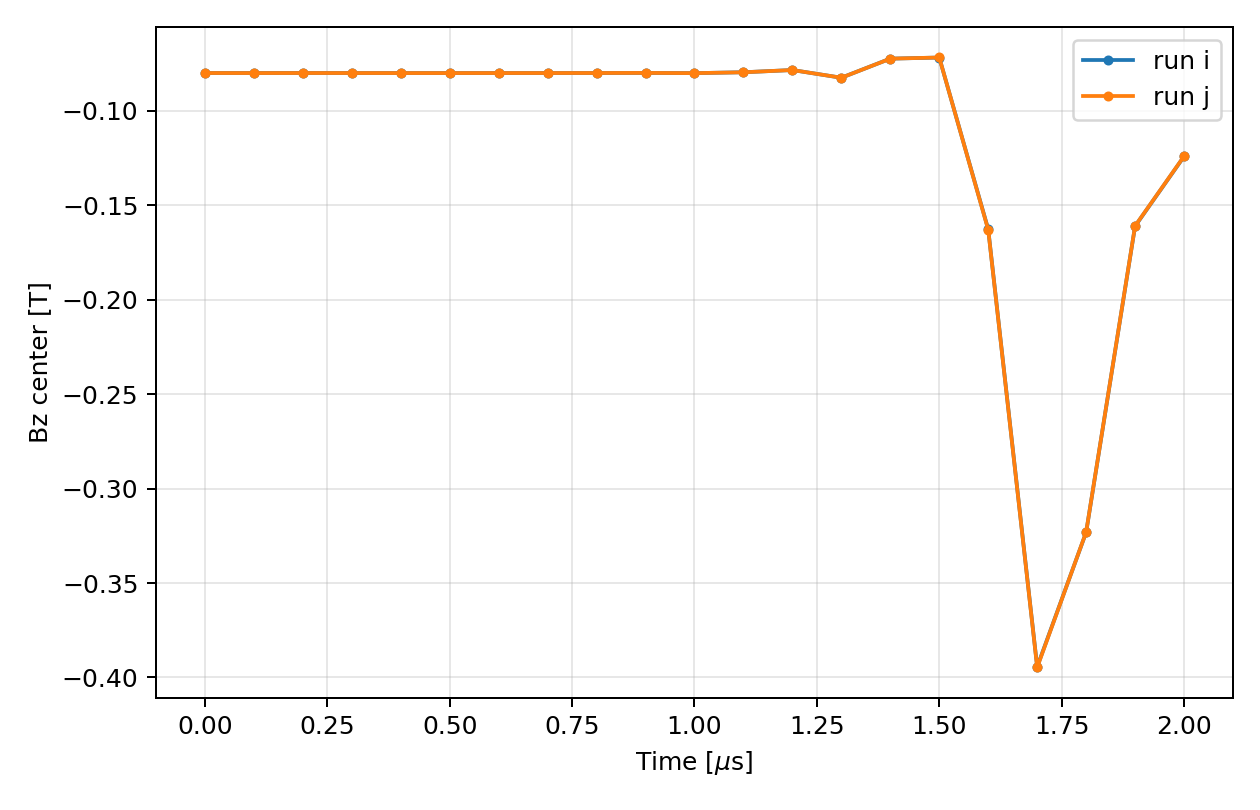
\includegraphics[
            width=\linewidth
        ]{img/audit/FRC_baseline_audit/Bz_center_vs_time.png}
    \end{minipage}
    \hfill
    \begin{minipage}{0.48\textwidth}
        \centering
        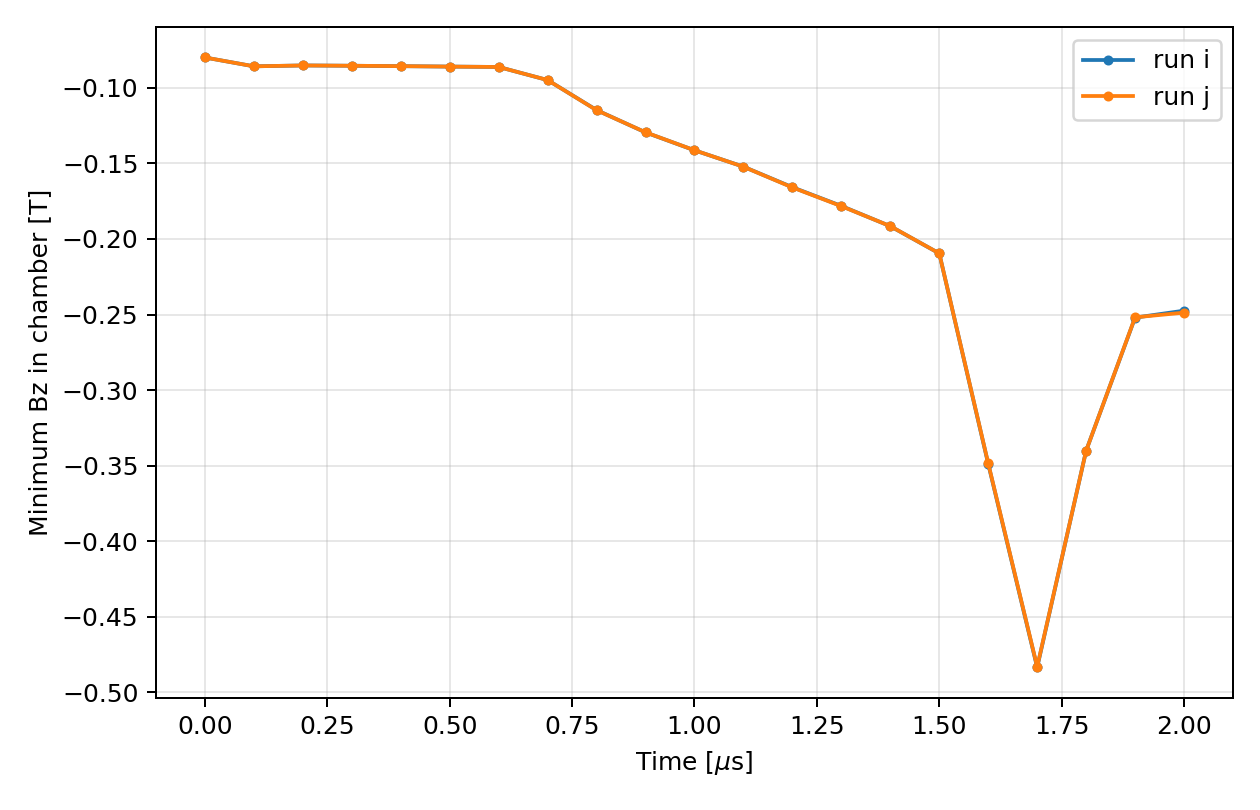
\includegraphics[
            width=\linewidth
        ]{img/audit/FRC_baseline_audit/Bz_min_vs_time.png}
    \end{minipage}

    \vspace{0.5em}

    \begin{minipage}{0.48\textwidth}
        \centering
        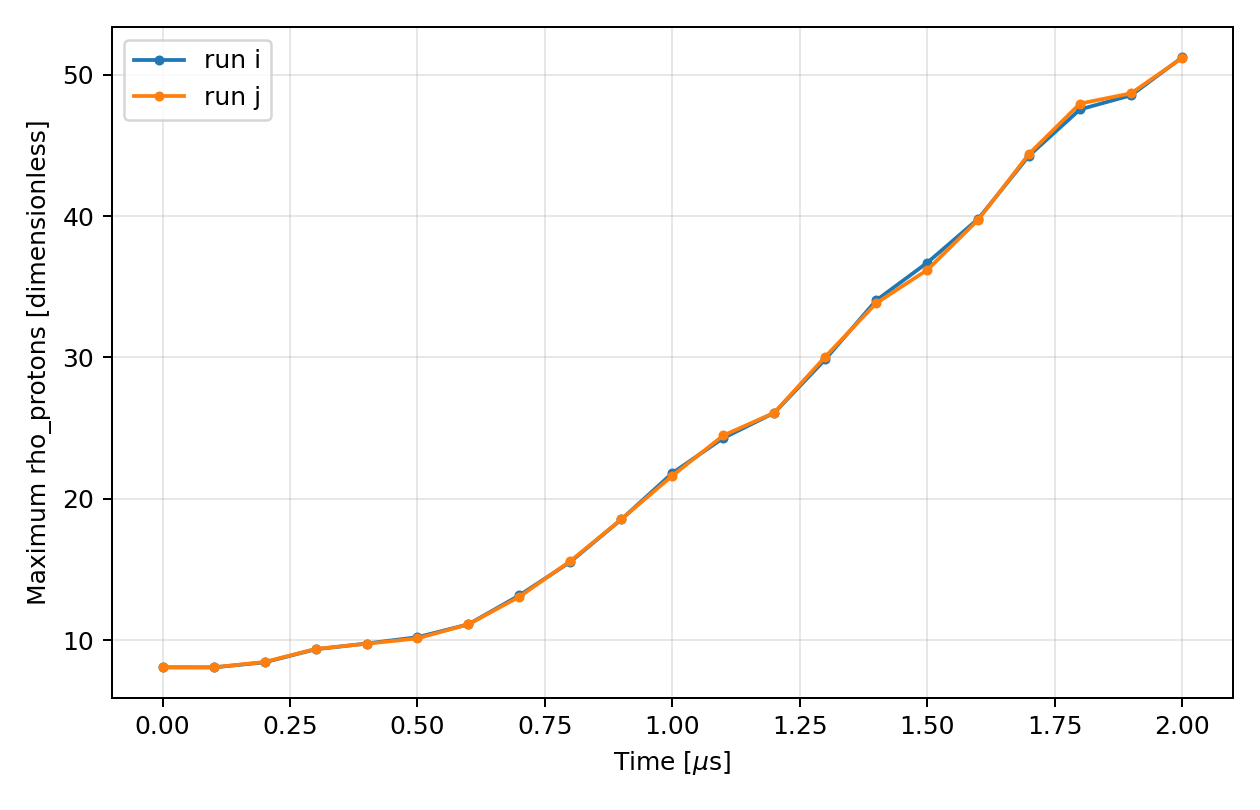
\includegraphics[
            width=\linewidth
        ]{img/audit/FRC_baseline_audit/rho_max_vs_time.png}
    \end{minipage}
    \hfill
    \begin{minipage}{0.48\textwidth}
        \centering
        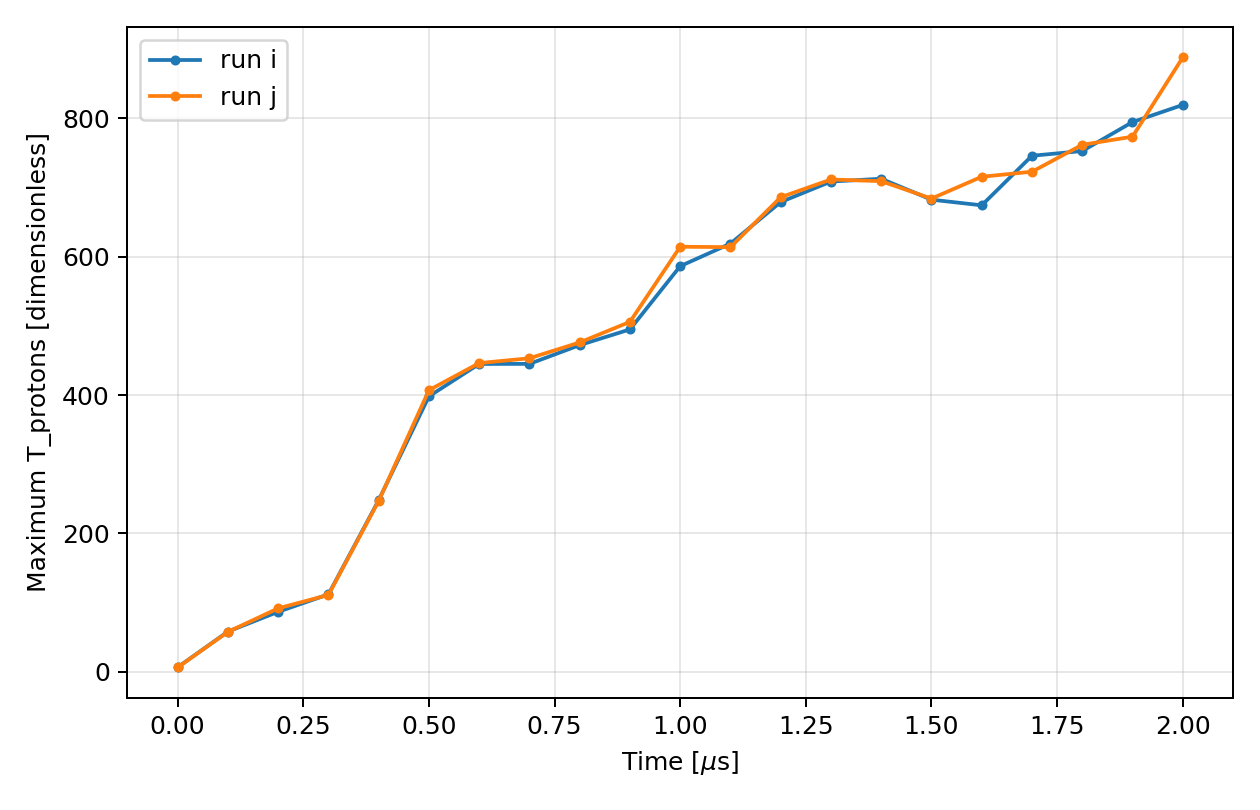
\includegraphics[
            width=\linewidth
        ]{img/audit/FRC_baseline_audit/Ti_max_vs_time.png}
    \end{minipage}

    \caption{
        Scalar evolution of the inherited runs \texttt{i} and \texttt{j}.
        The magnetic and density quantities show nearly identical
        macroscopic behavior. The pointwise maximum ion-temperature
        diagnostic is significantly more sensitive to the stochastic PIC
        realization and is therefore not considered a strong regression
        metric.
    }
    \label{fig:baseline_scalar_audit}
\end{figure}

The central axial magnetic field remains close to its initial value

\[
B_z\simeq -0.08~\mathrm{T}
\]

through much of the early evolution.

A strong transient develops between approximately

\[
1.5~\mu\mathrm{s}
\quad\mathrm{and}\quad
1.8~\mu\mathrm{s},
\]

with the central magnetic field reaching approximately

\[
B_{z,\mathrm{center}}
\simeq -0.395~\mathrm{T}.
\]

The minimum magnetic field inside the physical chamber reaches approximately

\[
B_{z,\min}
\simeq -0.483~\mathrm{T}.
\]

After this maximum compression, the central magnetic field partially relaxes,
reaching approximately

\[
B_{z,\mathrm{center}}
\simeq -0.124~\mathrm{T}
\]

at

\[
t=2~\mu\mathrm{s}.
\]

The maximum density diagnostic, in contrast, continues increasing through the
end of the available interval.

This indicates that the magnetic field begins to relax while the compressed
plasma structure remains present.


\subsection{Development of Magnetic-Field Reversal}

The \(x-z\) evolution of \(B_z\) is shown in
Figure~\ref{fig:bz_spatial_evolution}.

The plotted contour corresponds to

\[
B_z=0.
\]

This contour is used only as a \textbf{field-reversal proxy}.
It must not yet be identified rigorously with the FRC separatrix, since the
true magnetic topology is determined by the poloidal magnetic-flux function
rather than by the local condition \(B_z=0\) alone.

\begin{figure}[htbp]
    \centering

    \begin{minipage}{0.48\textwidth}
        \centering
        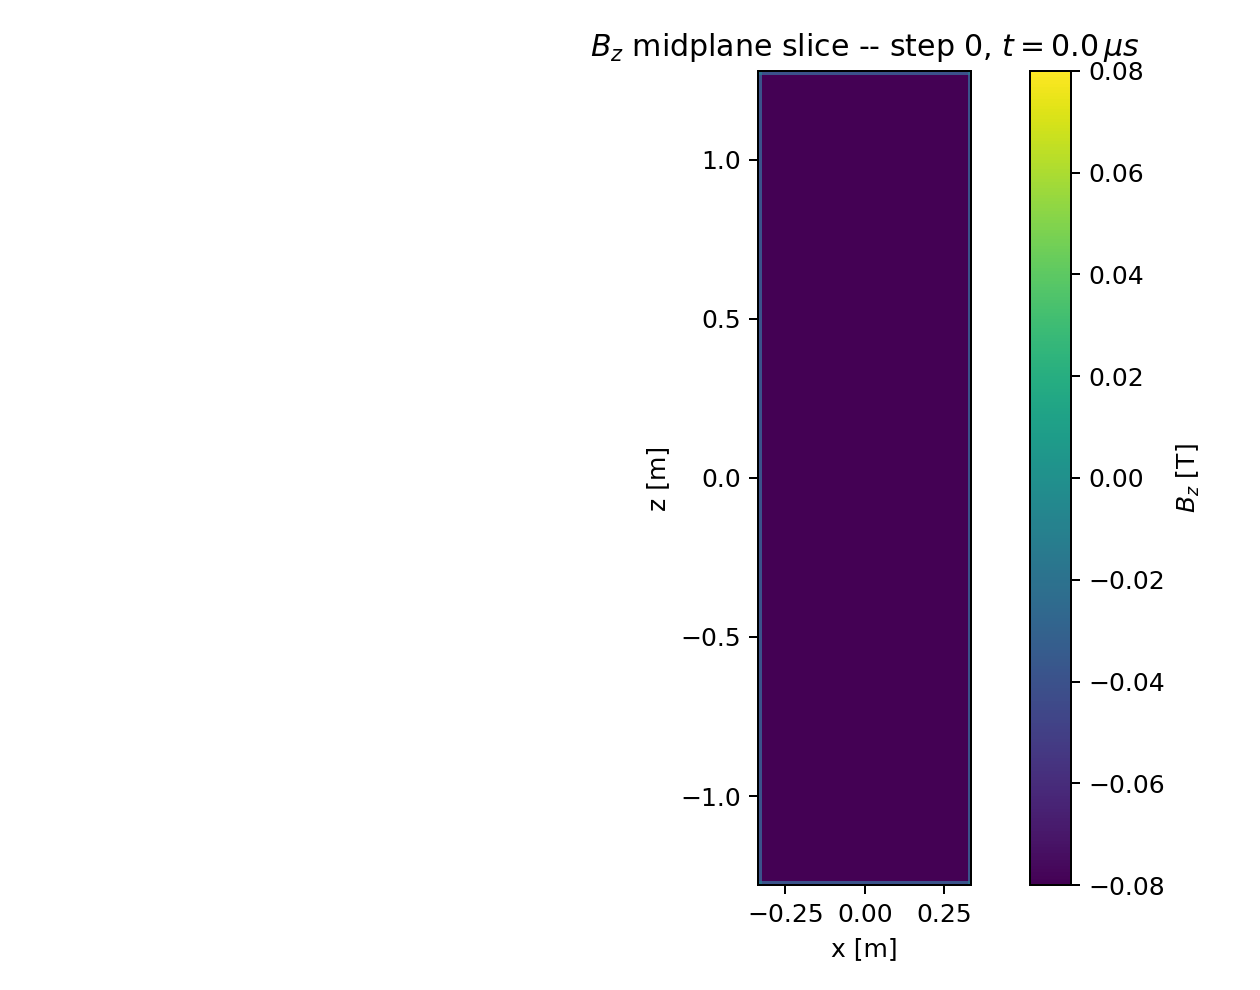
\includegraphics[
            width=\linewidth
        ]{img/audit/FRC_spatial_baseline/Bz_xz_step000000.png}
    \end{minipage}
    \hfill
    \begin{minipage}{0.48\textwidth}
        \centering
        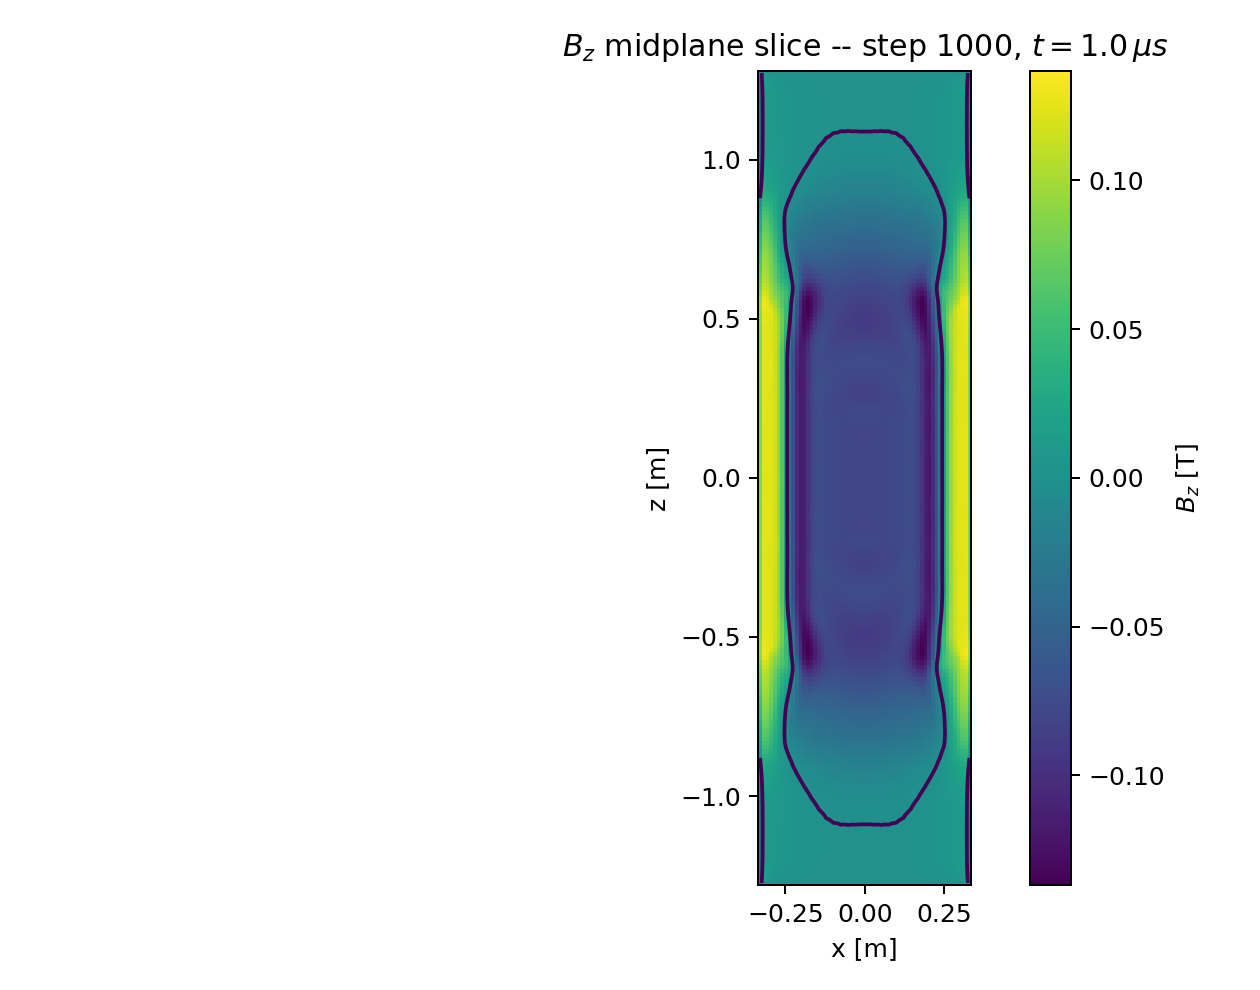
\includegraphics[
            width=\linewidth
        ]{img/audit/FRC_spatial_baseline/Bz_xz_step001000.png}
    \end{minipage}

    \vspace{0.5em}

    \begin{minipage}{0.48\textwidth}
        \centering
        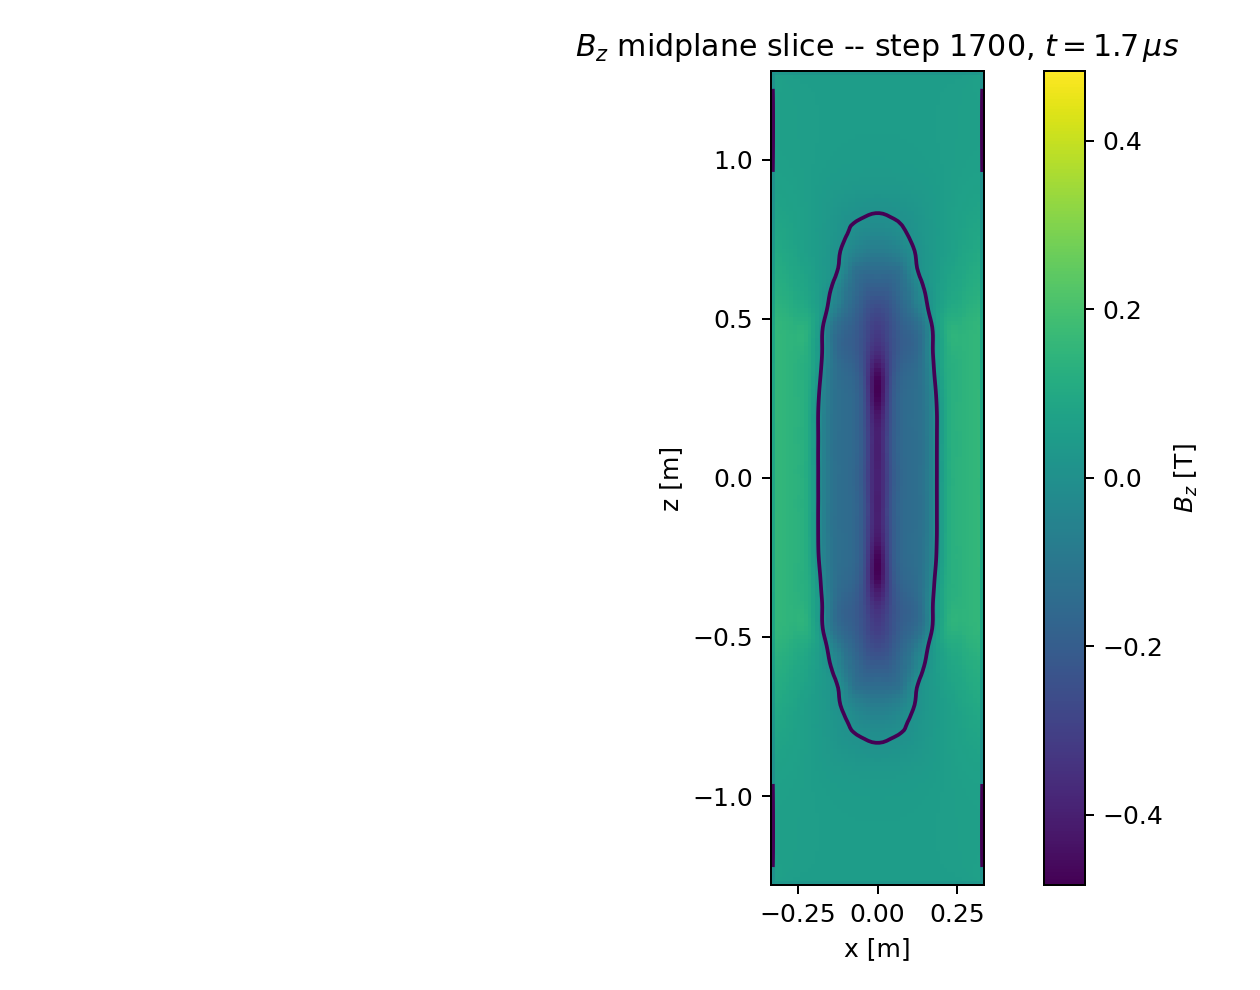
\includegraphics[
            width=\linewidth
        ]{img/audit/FRC_spatial_baseline/Bz_xz_step001700.png}
    \end{minipage}
    \hfill
    \begin{minipage}{0.48\textwidth}
        \centering
        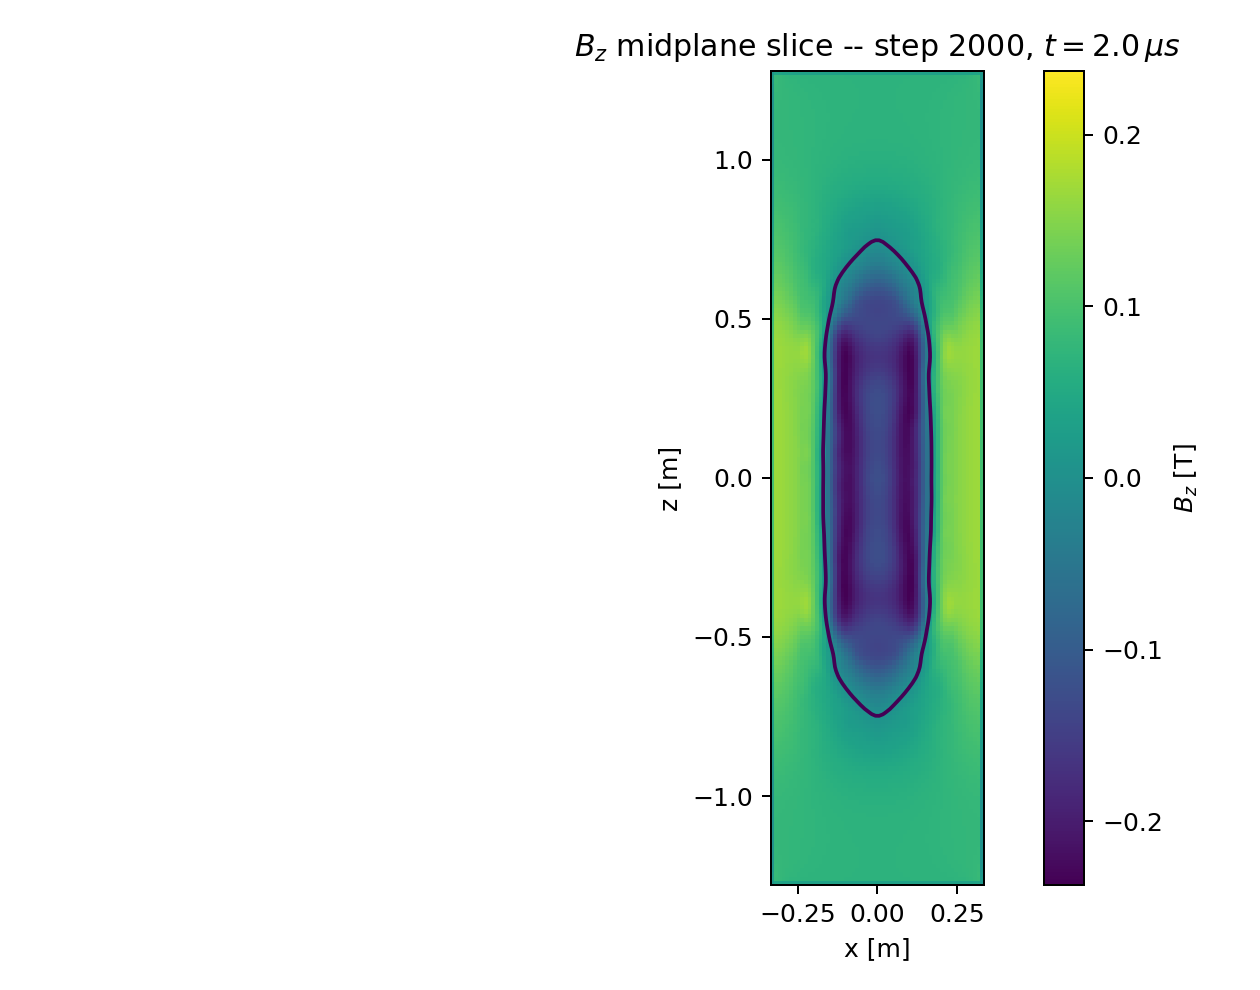
\includegraphics[
            width=\linewidth
        ]{img/audit/FRC_spatial_baseline/Bz_xz_step002000.png}
    \end{minipage}

    \caption{
        Evolution of \(B_z\) in the central \(x-z\) plane at
        \(t=0\), \(1.0\), \(1.7\), and \(2.0~\mu\mathrm{s}\).
        The dark contour represents \(B_z=0\) and is used as a
        field-reversal indicator, not yet as a rigorously reconstructed
        magnetic separatrix.
    }
    \label{fig:bz_spatial_evolution}
\end{figure}


\subsubsection{Initial state: \(t=0\)}

At the beginning of the simulation,

\[
B_z<0
\]

throughout the analyzed physical region.

The spatial range is approximately

\[
-0.08~\mathrm{T}
\leq
B_z
\leq
-0.02~\mathrm{T}.
\]

No \(B_z=0\) contour exists inside the analyzed region.

The configuration is therefore initially a biased axial magnetic field rather
than a field-reversed structure.


\subsubsection{Early reversal: \(t=1.0~\mu\mathrm{s}\)}

At \(t=1.0~\mu\mathrm{s}\), the magnetic field spans approximately

\[
-0.137~\mathrm{T}
\lesssim
B_z
\lesssim
+0.132~\mathrm{T}.
\]

Thus, positive and negative \(B_z\) regions coexist for the first time among
the representative snapshots.

A closed central \(B_z=0\) contour appears in the \(x-z\) plane.

The radial and axial magnetic profiles independently confirm the presence of
sign changes in \(B_z\).

This provides clear evidence that a coherent field-reversed region is already
developing by approximately

\[
t=1~\mu\mathrm{s}.
\]


\subsubsection{Strong compression: \(t=1.7~\mu\mathrm{s}\)}

The strongest magnetic compression within the available interval occurs near

\[
t=1.7~\mu\mathrm{s}.
\]

In the central \(x-z\) slice,

\[
B_{z,\min}
\simeq
-0.483~\mathrm{T},
\]

while the positive external field reaches approximately

\[
B_{z,\max}
\simeq
+0.155~\mathrm{T}.
\]

The resulting field-reversed region is substantially more compact than at
\(1.0~\mu\mathrm{s}\).

The central negative-\(B_z\) region remains approximately symmetric about

\[
x=0,\qquad z=0,
\]

and is surrounded by positive \(B_z\).

This spatial structure is consistent with a strongly compressed,
FRC-like magnetic configuration.


\subsubsection{Partial relaxation: \(t=2.0~\mu\mathrm{s}\)}

At the end of the inherited simulation,

\[
t=2.0~\mu\mathrm{s},
\]

the field-reversed structure remains clearly present.

The magnetic-field range in the central slice is approximately

\[
-0.237~\mathrm{T}
\lesssim
B_z
\lesssim
+0.168~\mathrm{T}.
\]

Compared with the state at \(1.7~\mu\mathrm{s}\), the negative central field
has weakened substantially.

However, the closed central \(B_z=0\) proxy remains visible.

The available data therefore suggest

\[
\boxed{
\text{formation}
\rightarrow
\text{strong compression}
\rightarrow
\text{partial magnetic relaxation}
}
\]

rather than disappearance of the field-reversed structure.


\subsection{Radial and Axial Magnetic Profiles}

The radial and axial profiles provide an independent view of the field
reversal.

\begin{figure}[htbp]
    \centering

    \begin{minipage}{0.49\textwidth}
        \centering
        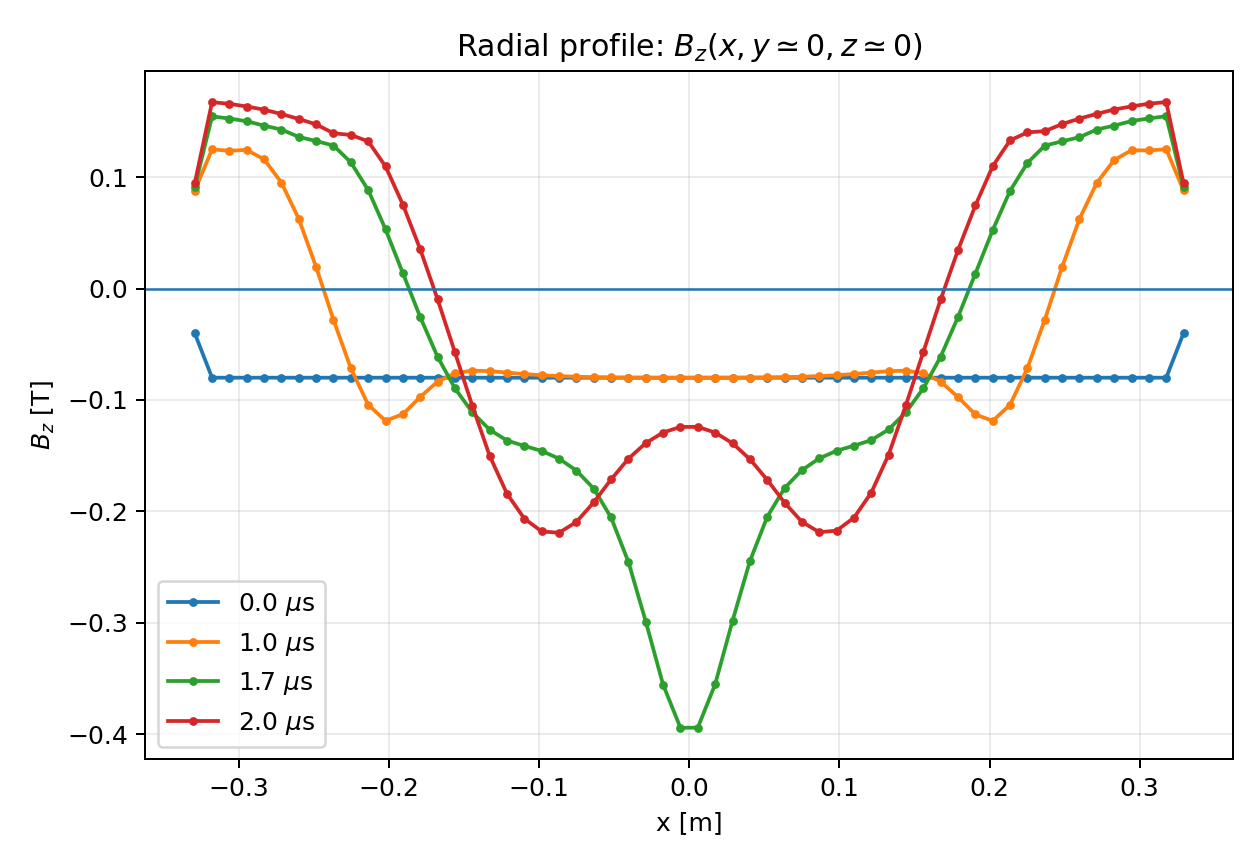
\includegraphics[
            width=\linewidth
        ]{img/audit/FRC_spatial_baseline/Bz_radial_profiles.png}
    \end{minipage}
    \hfill
    \begin{minipage}{0.49\textwidth}
        \centering
        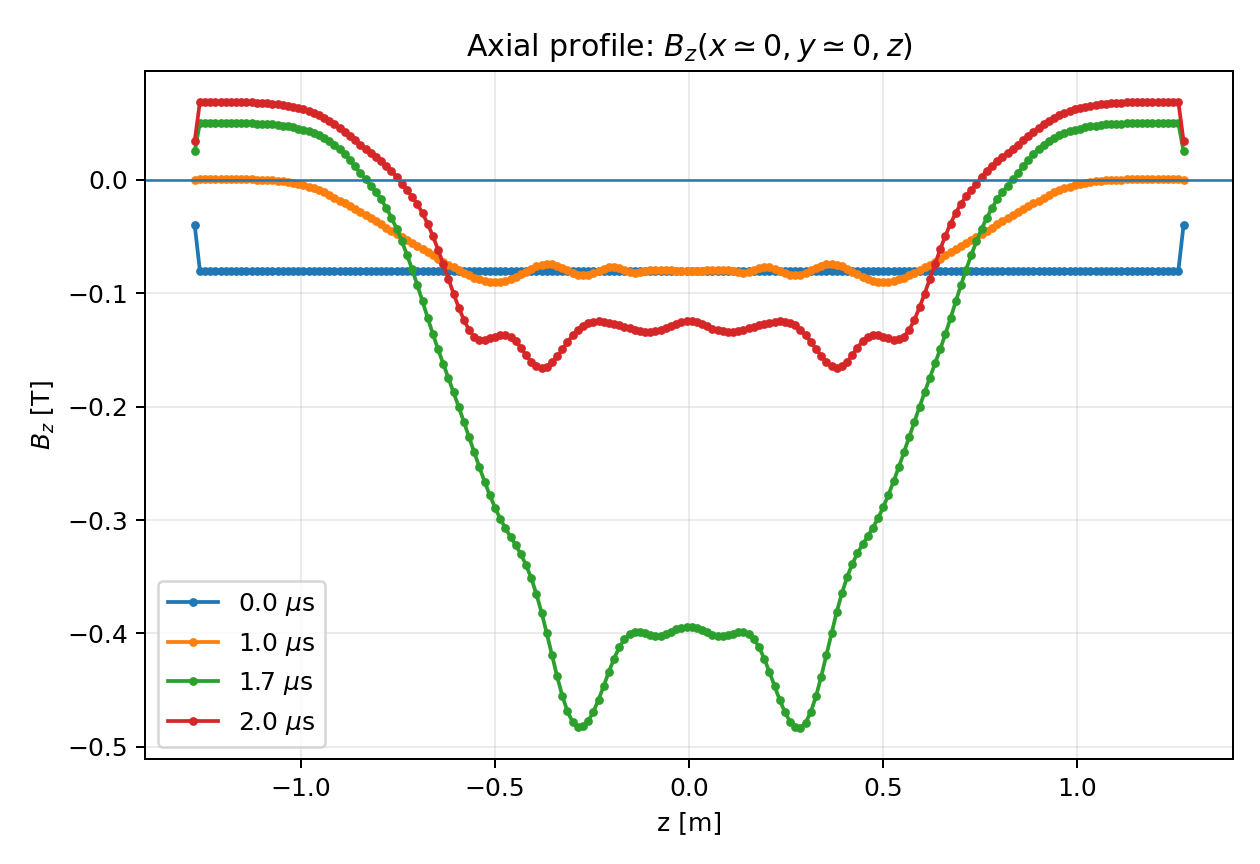
\includegraphics[
            width=\linewidth
        ]{img/audit/FRC_spatial_baseline/Bz_axial_profiles.png}
    \end{minipage}

    \caption{
        Radial and axial \(B_z\) profiles at representative times.
        The appearance of zero crossings along both directions confirms
        that the sign reversal observed in the two-dimensional maps is a
        spatially extended feature rather than an isolated cell-level
        fluctuation.
    }
    \label{fig:bz_profiles}
\end{figure}

Initially, the radial field is nearly uniform and negative.

By \(1.0~\mu\mathrm{s}\), two radial zero crossings appear, separating the
negative interior from the positive external region.

At \(1.7~\mu\mathrm{s}\), the radial profile develops its deepest central
minimum,

\[
B_z(x\simeq0)
\simeq
-0.40~\mathrm{T},
\]

and remains approximately symmetric with respect to \(x=0\).

The axial profile shows the same qualitative evolution.

At the later times, the central negative-field region is bounded axially by
positive-field regions, demonstrating that the reversal is extended in both
the radial and axial directions.

These profiles strengthen the interpretation that the observed structure is
macroscopic and coherent rather than a consequence of local PIC noise.


\subsection{Density Compression}

The corresponding evolution of the ion-density diagnostic is shown in
Figure~\ref{fig:rho_spatial_evolution}.

\begin{figure}[htbp]
    \centering

    \begin{minipage}{0.48\textwidth}
        \centering
        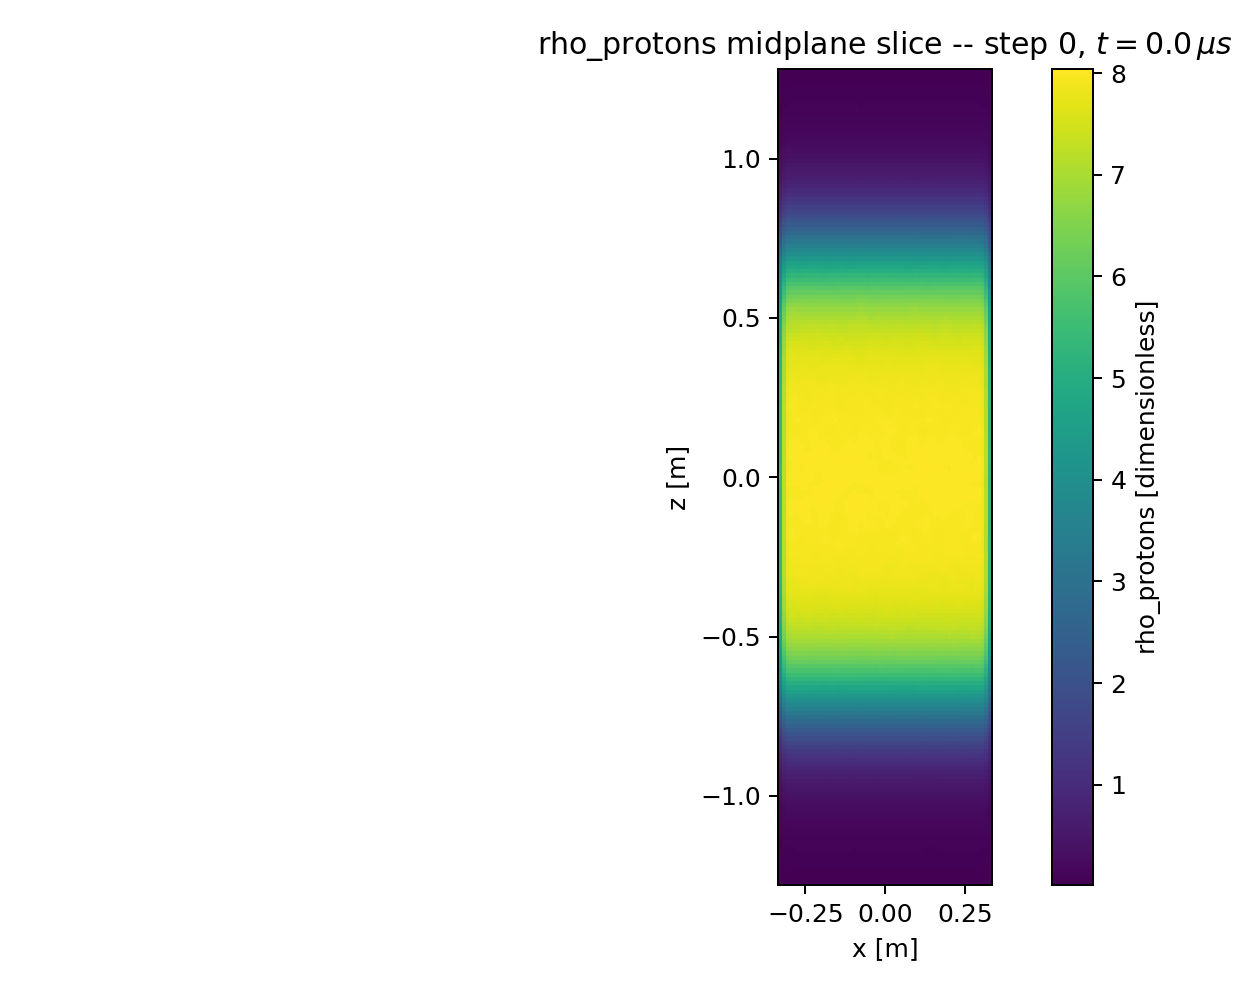
\includegraphics[
            width=\linewidth
        ]{img/audit/FRC_spatial_baseline/rho_xz_step000000.png}
    \end{minipage}
    \hfill
    \begin{minipage}{0.48\textwidth}
        \centering
        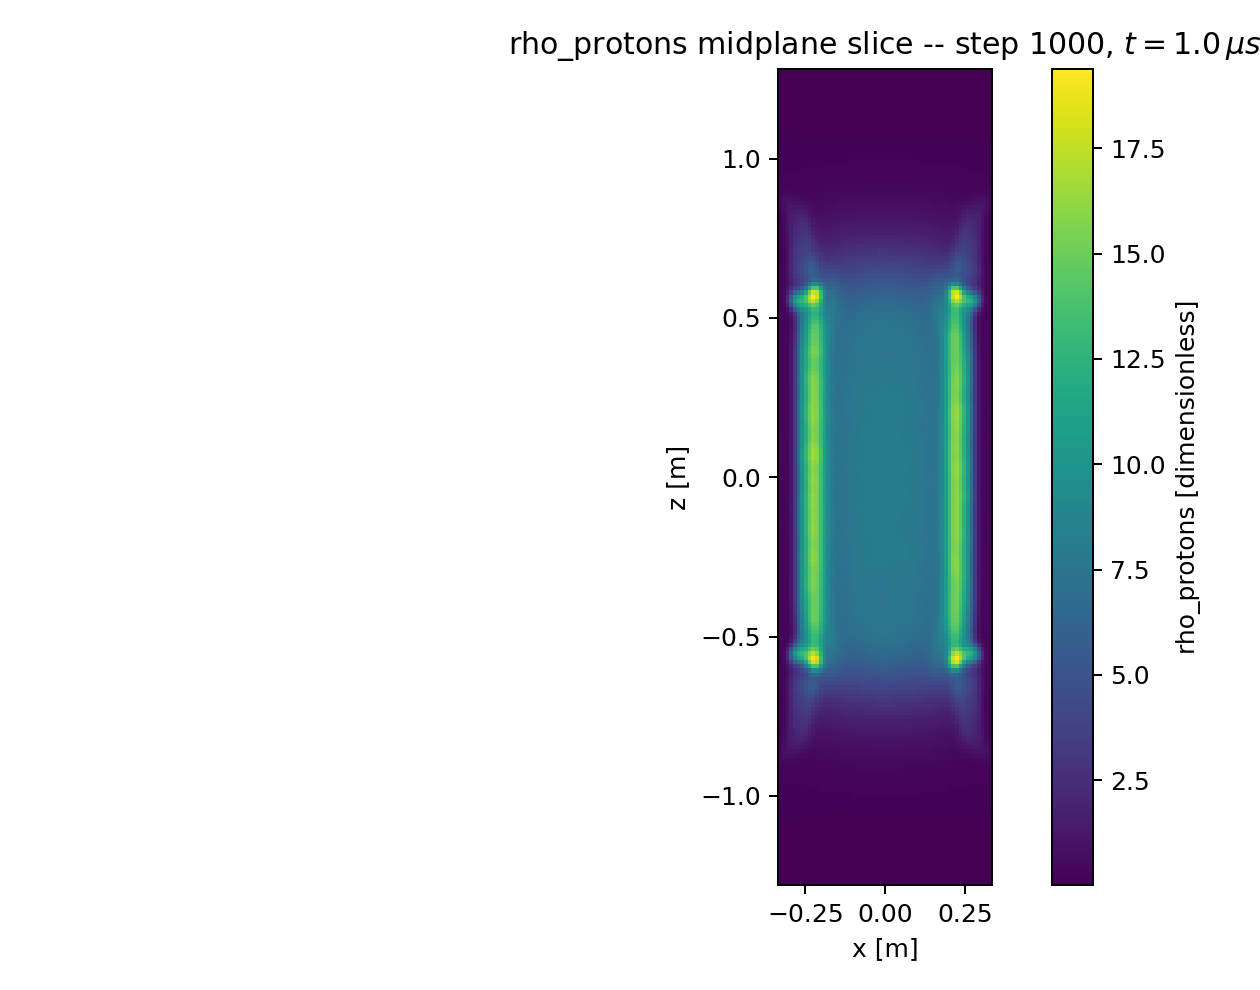
\includegraphics[
            width=\linewidth
        ]{img/audit/FRC_spatial_baseline/rho_xz_step001000.png}
    \end{minipage}

    \vspace{0.5em}

    \begin{minipage}{0.48\textwidth}
        \centering
        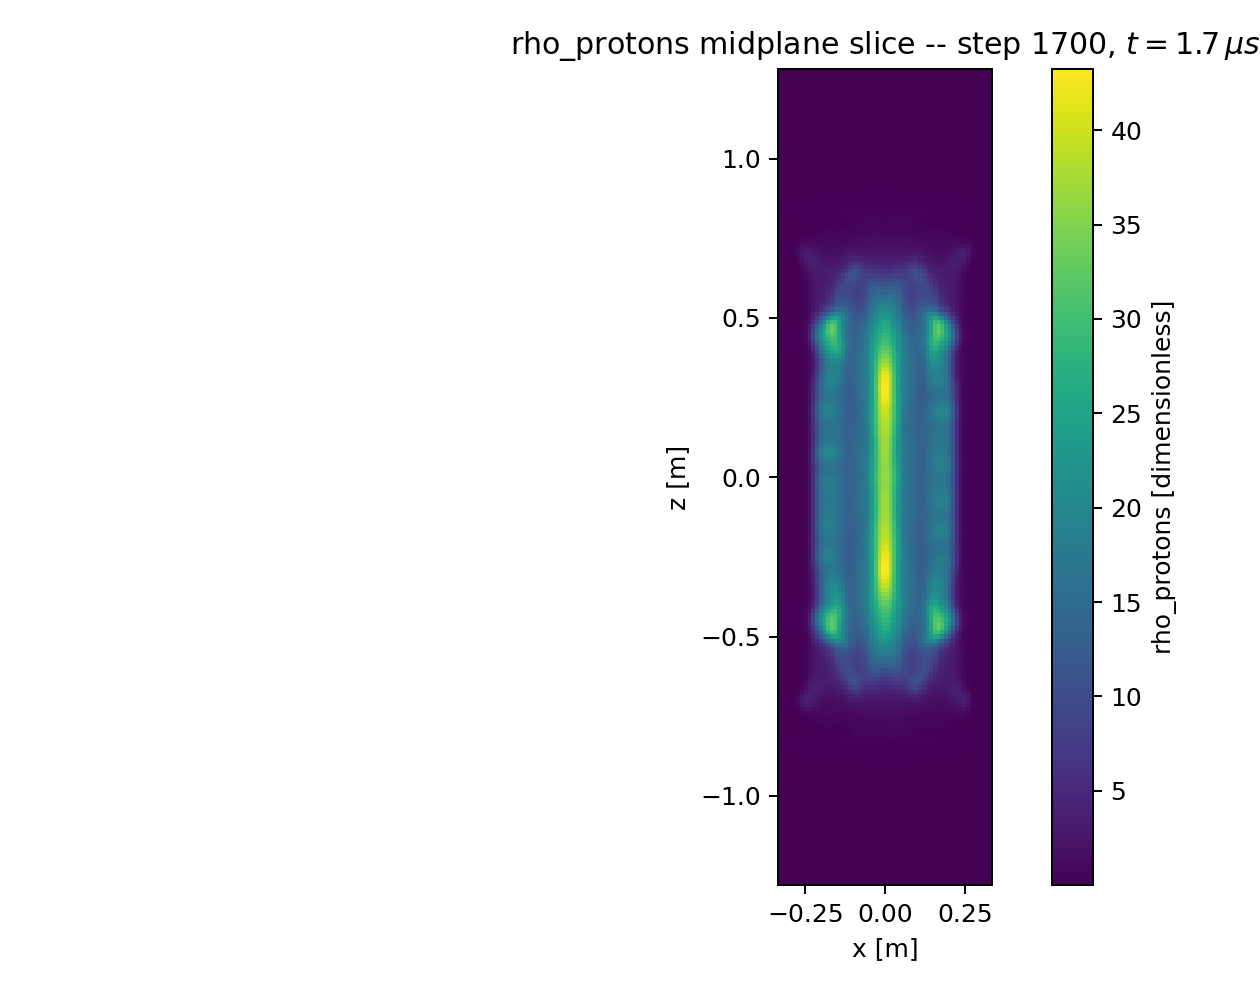
\includegraphics[
            width=\linewidth
        ]{img/audit/FRC_spatial_baseline/rho_xz_step001700.png}
    \end{minipage}
    \hfill
    \begin{minipage}{0.48\textwidth}
        \centering
        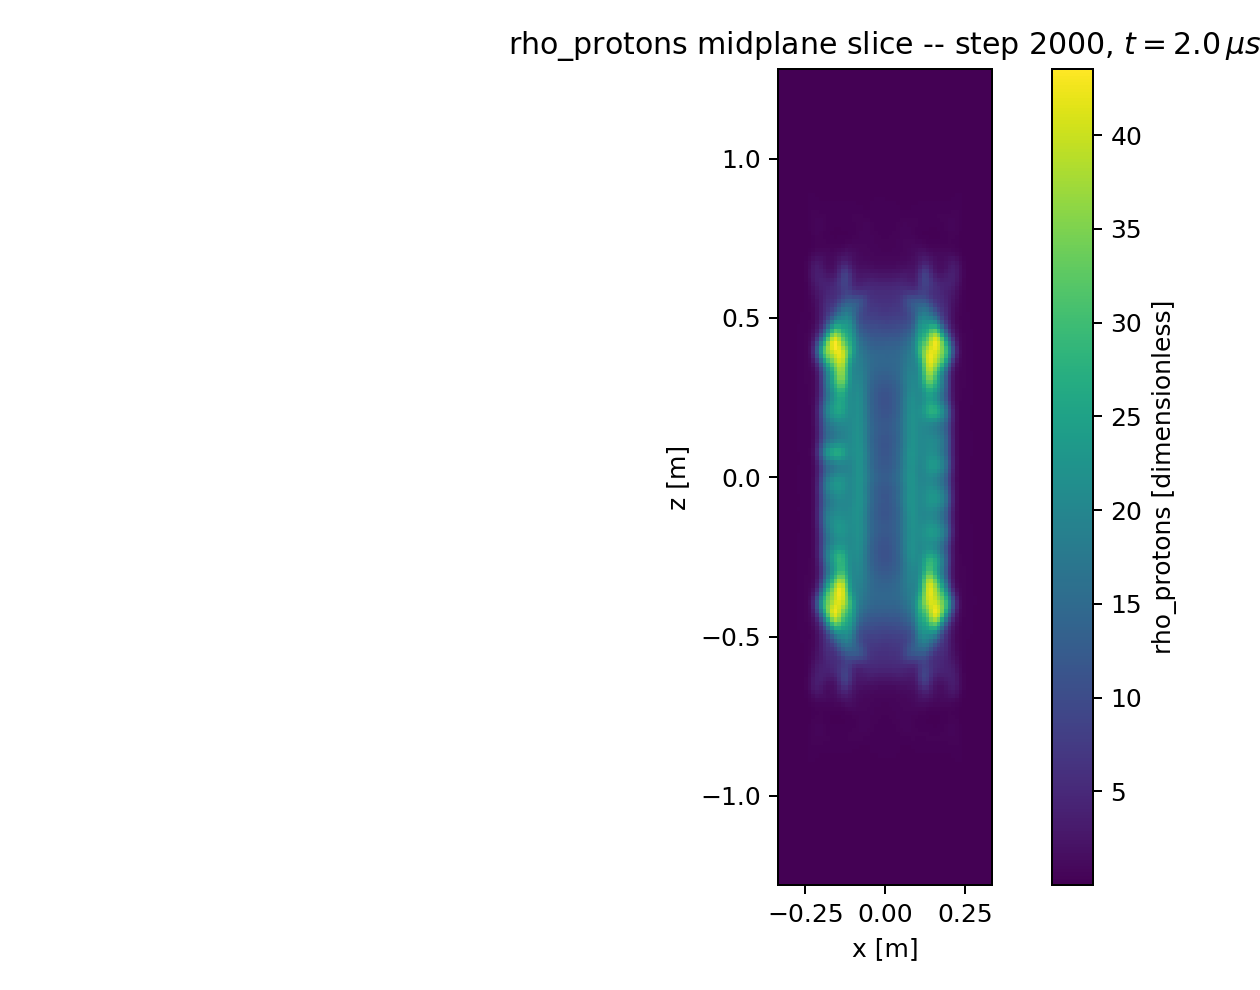
\includegraphics[
            width=\linewidth
        ]{img/audit/FRC_spatial_baseline/rho_xz_step002000.png}
    \end{minipage}

    \caption{
        Evolution of the stored \texttt{rho\_protons} diagnostic in the
        central \(x-z\) plane. A substantial spatial redistribution and
        compression of the plasma accompanies the development of the
        reversed-field structure.
    }
    \label{fig:rho_spatial_evolution}
\end{figure}

At \(t=0\), the plasma density is broadly distributed through the central
axial region.

By \(1.0~\mu\mathrm{s}\), the density distribution develops strong
off-axis structures and enhanced regions near the radial edges of the plasma.

At \(1.7~\mu\mathrm{s}\), the plasma is substantially compressed and a strong
central density enhancement is visible.

The maximum stored density in this \(x-z\) slice increases from approximately

\[
8.0
\]

at the initial time to approximately

\[
43.2
\]

at \(1.7~\mu\mathrm{s}\).

At \(2.0~\mu\mathrm{s}\), the slice maximum remains approximately

\[
43.5,
\]

even though the central magnetic field has already begun to relax.

Therefore, the density compression persists longer than the strongest
magnetic-field transient in the current interval.

The maximum density obtained from the full three-dimensional domain is larger,
approximately

\[
51,
\]

indicating that the global density maximum is not necessarily located in the
central \(y\simeq0\) plane.

This may become relevant in future three-dimensional symmetry and instability
studies, but it is not necessary to pursue further during the present
takeover audit.


\subsection{Important Limitation: \(B_z=0\) Is Not Yet the Separatrix}

The spatial analysis provides strong evidence for the development of a
field-reversed, FRC-like magnetic structure.

However, the contour

\[
B_z=0
\]

should not yet be interpreted as the exact FRC separatrix.

For an axisymmetric magnetic configuration, the magnetic topology is more
properly described using the poloidal magnetic-flux function

\[
\psi(r,z).
\]

Identification of

\begin{itemize}
    \item the O-point,
    \item the X-points,
    \item closed magnetic-flux surfaces,
    \item the separatrix,
    \item the separatrix radius \(R_s\),
    \item and the separatrix length \(L_s\)
\end{itemize}

should therefore ultimately be based on \(\psi\) or an equivalent
field-line/flux reconstruction.

The present \(B_z=0\) contour is sufficient as a practical proxy for the
baseline audit, but it should not replace a future magnetic-topology
diagnostic.


\section{Final Interpretation of the Inherited Formation Baseline}

The combined scalar and spatial audit supports the following interpretation
of the inherited 2000-step simulation.

\begin{enumerate}[label=\arabic*.]

    \item The simulation begins from a negative axial bias magnetic field with
    no field reversal.

    \item A coherent field-reversed region develops during the first
    microsecond.

    \item By approximately
    \[
    t=1.0~\mu\mathrm{s},
    \]
    positive and negative \(B_z\) regions coexist and a closed central
    \(B_z=0\) contour is visible.

    \item The strongest compression occurs near
    \[
    t=1.7~\mu\mathrm{s},
    \]
    when both the magnitude of the reversed magnetic field and the plasma
    density are strongly enhanced.

    \item At
    \[
    t=2.0~\mu\mathrm{s},
    \]
    the magnetic field has partially relaxed, but the reversed-field
    structure and strongly compressed plasma remain present.

    \item Independent particle realizations \texttt{i} and \texttt{j}
    reproduce essentially the same macroscopic magnetic and density
    evolution.

\end{enumerate}

The inherited simulation therefore provides a useful and nontrivial
regression baseline.

It is not merely a test that WarpX executes successfully; it contains a
reproducible sequence of

\[
\boxed{
\text{field reversal}
\rightarrow
\text{plasma compression}
\rightarrow
\text{partial magnetic relaxation}
}
\]

that can be used to validate future changes to the workflow.


\subsection{What Has Been Established}

At the end of the takeover audit, the following points are considered
established:

\begin{itemize}

    \item The exact inherited WarpX executable and source commit have been
    identified.

    \item The apparent WarpX \texttt{dirty} state is associated with
    line-ending differences rather than identified solver modifications.

    \item The inherited Slurm execution configuration has been documented.

    \item Runs \texttt{i} and \texttt{j} use the same physical and numerical
    inputs.

    \item Their outputs are not bitwise identical because the PIC particle
    realization is stochastic.

    \item Their macroscopic magnetic and density evolution is nevertheless
    highly reproducible.

    \item The existing run evolves for
    \[
    2~\mu\mathrm{s},
    \]
    which is shorter than the imposed
    \[
    4~\mu\mathrm{s}
    \]
    field-rise time.

    \item The existing simulation should therefore be treated as a
    \textbf{computational regression baseline}, rather than as the final
    scientific formation case.

    \item The baseline produces a coherent, spatially resolved,
    field-reversed FRC-like structure.

\end{itemize}


\section{Baseline Regression Quantities}

The future framework should reproduce the macroscopic evolution of this
baseline rather than attempt binary equality of the WarpX plotfiles.

The first regression quantities should include

\[
B_{z,\mathrm{center}}(t),
\]

\[
B_{z,\min}(t),
\]

\[
B_{z,\max}(t),
\]

\[
\rho_{\mathrm{center}}(t),
\]

and

\[
\rho_{\max}(t).
\]

Spatial regression should additionally verify the qualitative presence and
approximate geometry of the reversed-field region at representative times.

Pointwise quantities such as

\[
T_{i,\max}
\]

should not initially be used as strict pass/fail quantities because they are
significantly more sensitive to local PIC noise.

More robust temperature metrics should later use

\begin{itemize}
    \item central averages,
    \item spatial averages,
    \item volume-weighted quantities,
    \item or high-percentile values rather than absolute maxima.
\end{itemize}


\section{Transition from Audit to Framework Development}

The inherited baseline is now sufficiently characterized to begin independent
framework development.

Further analysis of the old run should only be added when required for a
specific scientific or regression diagnostic.

The next project phase is therefore

\[
\boxed{\text{Framework v0.1}}
\]

rather than continued open-ended investigation of the inherited workflow.

The development sequence will be

\[
\boxed{
\text{freeze reference}
\rightarrow
\text{framework v0.1}
\rightarrow
\text{smoke test}
\rightarrow
\text{2000-step regression}
\rightarrow
\text{scientific formation baseline}
}
\]


\subsection{Immediate Framework Objectives}

The first framework version should remain deliberately small.

Its purpose is to introduce controlled case definition and provenance without
changing the validated physics.

The first implementation should provide:

\begin{enumerate}[label=\arabic*.]

    \item A structured case configuration separating
    \begin{itemize}
        \item physical parameters,
        \item geometry,
        \item numerical parameters,
        \item diagnostics,
        \item and HPC/runtime parameters.
    \end{itemize}

    \item Automated validation of basic consistency conditions.

    \item Generation of a readable WarpX input file.

    \item A controlled Slurm submission script.

    \item Automatic creation of a run directory.

    \item A run manifest containing
    \begin{itemize}
        \item case name,
        \item parameter values,
        \item framework Git commit,
        \item WarpX version,
        \item WarpX executable checksum,
        \item Slurm job ID,
        \item MPI/OpenMP configuration,
        \item and output paths.
    \end{itemize}

    \item Automatic preservation of
    \texttt{warpx\_used\_inputs}.

    \item Reuse of the existing baseline-analysis tools for regression
    comparison.

\end{enumerate}


\subsection{First Independent Execution}

The first independently controlled WarpX execution should be a short smoke
test rather than a full 2000-step production run.

The smoke test should preserve the important model configuration while using

\begin{itemize}
    \item approximately 10--20 timesteps,
    \item minimal diagnostic output,
    \item no large full-state checkpoints unless explicitly needed,
    \item and a short Slurm walltime.
\end{itemize}

Its purpose is only to verify

\[
\text{config}
\rightarrow
\text{generated input}
\rightarrow
\text{Slurm}
\rightarrow
\text{WarpX}
\rightarrow
\text{output}
\]

under the new framework.


\subsection{Regression Reproduction}

After the smoke test succeeds, the complete inherited 2000-step configuration
will be reproduced independently.

Success will be evaluated using the baseline quantities established during
the present audit.

The target is not byte-level equality.

Instead, the new run must reproduce the same macroscopic sequence:

\[
\text{initial bias}
\rightarrow
\text{field reversal}
\rightarrow
\text{strong compression}
\rightarrow
\text{partial relaxation}.
\]

Only after this regression test is passed should numerical optimization or
physical changes be introduced.


\subsection{Scientific Formation Baseline}

The present inherited simulation ends at

\[
t=2~\mu\mathrm{s},
\]

whereas the external field reaches its nominal peak only at

\[
t_{\mathrm{peak}}
=
4~\mu\mathrm{s}.
\]

Therefore, a later scientific formation baseline must extend at least through

\[
t=4~\mu\mathrm{s},
\]

and probably beyond this time.

That longer simulation will be used to study

\begin{itemize}
    \item completion of FRC formation,
    \item post-formation magnetic topology,
    \item density and temperature evolution,
    \item flux retention,
    \item particle losses,
    \item energy evolution,
    \item lifetime,
    \item and eventually stability.
\end{itemize}

At that stage, magnetic-flux reconstruction should be added in order to
identify the true separatrix and calculate quantities such as

\[
R_s,\qquad
L_s,\qquad
E=\frac{L_s}{2R_s},
\]

as well as trapped poloidal flux.


\section{Status at the End of the Takeover Audit}

The takeover phase can now be considered successfully completed.

The project has progressed from

\begin{quote}
an inherited WarpX input and a collection of existing output directories
\end{quote}

to

\begin{quote}
a documented, physically characterized, quantitatively reproducible
reference case that can serve as the first regression test of a new FRC
simulation framework.
\end{quote}

The immediate focus now shifts from understanding the inherited workflow to
building an independently controlled and reproducible research framework.

\end{document}
